% Remember to save this document with a .Rnw file ending,
% before you use the engine Knitr to compile it.
% *** !TEX TS-program = pdflatexmk
% arara: clean: { files: [thesis.aux, thesis.bbl, thesis.blg, thesis.dvi, thesis.fdb_latexmk, thesis.fls, thesis.idx, thesis.ilg, thesis.ind, thesis.lof, thesis.log, thesis.lot, thesis.nlo, thesis.nls, thesis.out, thesis.pdf, thesis.ps, thesis.toc]}
% arara: latex:  { shell: yes }
% arara: bibtex
% arara: nomencl
% arara: latex
% arara: makeindex
% arara: latex:  { shell: yes }
% arara: dvips
% arara: ps2pdf

% ******************************* PhD Thesis Template **************************
% Please have a look at the README.md file for info on how to use the template

\documentclass[a4paper,12pt,times,authoryear,oneside,openright,online,index]{Classes/PhDThesisPSnPDF}\usepackage[]{graphicx}\usepackage[]{color}
%% maxwidth is the original width if it is less than linewidth
%% otherwise use linewidth (to make sure the graphics do not exceed the margin)
\makeatletter
\def\maxwidth{ %
  \ifdim\Gin@nat@width>\linewidth
    \linewidth
  \else
    \Gin@nat@width
  \fi
}
\makeatother

\definecolor{fgcolor}{rgb}{0.345, 0.345, 0.345}
\newcommand{\hlnum}[1]{\textcolor[rgb]{0.686,0.059,0.569}{#1}}%
\newcommand{\hlstr}[1]{\textcolor[rgb]{0.192,0.494,0.8}{#1}}%
\newcommand{\hlcom}[1]{\textcolor[rgb]{0.678,0.584,0.686}{\textit{#1}}}%
\newcommand{\hlopt}[1]{\textcolor[rgb]{0,0,0}{#1}}%
\newcommand{\hlstd}[1]{\textcolor[rgb]{0.345,0.345,0.345}{#1}}%
\newcommand{\hlkwa}[1]{\textcolor[rgb]{0.161,0.373,0.58}{\textbf{#1}}}%
\newcommand{\hlkwb}[1]{\textcolor[rgb]{0.69,0.353,0.396}{#1}}%
\newcommand{\hlkwc}[1]{\textcolor[rgb]{0.333,0.667,0.333}{#1}}%
\newcommand{\hlkwd}[1]{\textcolor[rgb]{0.737,0.353,0.396}{\textbf{#1}}}%

\usepackage{framed}
\makeatletter
\newenvironment{kframe}{%
 \def\at@end@of@kframe{}%
 \ifinner\ifhmode%
  \def\at@end@of@kframe{\end{minipage}}%
  \begin{minipage}{\columnwidth}%
 \fi\fi%
 \def\FrameCommand##1{\hskip\@totalleftmargin \hskip-\fboxsep
 \colorbox{shadecolor}{##1}\hskip-\fboxsep
     % There is no \\@totalrightmargin, so:
     \hskip-\linewidth \hskip-\@totalleftmargin \hskip\columnwidth}%
 \MakeFramed {\advance\hsize-\width
   \@totalleftmargin\z@ \linewidth\hsize
   \@setminipage}}%
 {\par\unskip\endMakeFramed%
 \at@end@of@kframe}
\makeatother

\definecolor{shadecolor}{rgb}{.97, .97, .97}
\definecolor{messagecolor}{rgb}{0, 0, 0}
\definecolor{warningcolor}{rgb}{1, 0, 1}
\definecolor{errorcolor}{rgb}{1, 0, 0}
\newenvironment{knitrout}{}{} % an empty environment to be redefined in TeX

\usepackage{alltt}
% I copied PhDThesisPSnPDF.cls to /usr/local/texlive/2012/texmf/tex/latex
% execute $ sudo texhash
%\documentclass[a4paper,12pt,times,numbered,print,index]{PhDThesisPSnPDF}

% ******************************************************************************
% ******************************* Class Options ********************************
% *********************** See README for more details **************************
% ******************************************************************************

% `a4paper'(The University of Cambridge PhD thesis guidelines recommends a page
% size a4 - default option) or `a5paper': A5 Paper size is also allowed as per
% the Cambridge University Engineering Deparment guidelines for PhD thesis
%
% `11pt' or `12pt'(default): Font Size 10pt is NOT recommended by the University
% guidelines
%
% `oneside' or `twoside'(default): Printing double side (twoside) or single
% side.
%
% `print': Use `print' for print version with appropriate margins and page
% layout. Leaving the options field blank will activate Online version.
%
% `index': For index at the end of the thesis
%
% `draft': For draft mode without loading any images (same as draft in book)
%
% `draftmode': Special draft mode with line numbers, images, and water mark with
% timestamp and custom text. Position of the text can also be modified.
%
% `abstract': To generate only the title page and abstract page with
% dissertation title and name, to submit to the Student Registry
%
% `chapter`: This option enables only the specified chapter and it's references
%  Useful for review and corrections.
%
% ************************* Custom Page Margins ********************************
%
% `custommargin`: Use `custommargin' in options to activate custom page margins,
% which can be defined in the preamble.tex. Custom margin will override
% print/online margin setup.
%
% *********************** Choosing the Fonts in Class Options ******************
%
% `times' : Times font with math support. (The Cambridge University guidelines
% recommend using times)
%
% `fourier': Utopia Font with Fourier Math font (Font has to be installed)
%            It's a free font.
%
% `customfont': Use `customfont' option in the document class and load the
% package in the preamble.tex
%
% default or leave empty: `Latin Modern' font will be loaded.
%
% ********************** Choosing the Bibliography style ***********************
%
% `authoryear': For author-year citation eg., Krishna (2013)
%
% `numbered': (Default Option) For numbered and sorted citation e.g., [1,5,2]
%
% `custombib': Define your own bibliography style in the `preamble.tex' file.
%              `\RequirePackage[square, sort, numbers, authoryear]{natbib}'.
%              This can be also used to load biblatex instead of natbib
%              (See Preamble)
%
% **************************** Choosing the Page Style *************************
%
% `default (leave empty)': For Page Numbers in Header (Left Even, Right Odd) and
% Chapter Name in Header (Right Even) and Section Name (Left Odd). Blank Footer.
%
% `PageStyleI': Chapter Name next & Page Number on Even Side (Left Even).
% Section Name & Page Number in Header on Odd Side (Right Odd). Footer is empty.
%
% `PageStyleII': Chapter Name on Even Side (Left Even) in Header. Section Number
% and Section Name in Header on Odd Side (Right Odd). Page numbering in footer


% ********************************** Preamble **********************************
% Preamble: Contains packages and user-defined commands and settings
% ******************************************************************************
% ****************************** Custom Margin *********************************

% Add `custommargin' in the document class options to use this section
% Set {innerside margin / outerside margin / topmargin / bottom margin}  and
% other page dimensions
\ifsetCustomMargin
  \RequirePackage[left=42mm,right=35mm,top=25mm,bottom=20mm]{geometry}
  \setFancyHdr % To apply fancy header after geometry package is loaded
\fi

% *****************************************************************************
% ******************* Fonts (like different typewriter fonts etc.)*************

% Add `customfont' in the document class option to use this section

\ifsetCustomFont
  % Set your custom font here and use `customfont' in options. Leave empty to
  % load computer modern font (default LaTeX font).
  \RequirePackage{helvet}
\fi

% *****************************************************************************
% **************************** Custom Packages ********************************
\usepackage{import}

%\usepackage{comment}

\usepackage{epigraph}

%% ---- package for formatting code with line numbers
\usepackage{fancyvrb} %% for verbatim text

\usepackage{ulem} % more underlining and other font effects

% ************************** Custom Floats **********************************
\usepackage{float}
\floatstyle{ruled}
\newfloat{cmd}{htb}{loc}[chapter]
\floatname{cmd}{Command}
% **** **** **** **** **** **** **** ****

%% ---- provides "\rowcolors" command
\usepackage[dvipsnames,table]{xcolor}

\usepackage{subcaption}

% ---- the following package call ensures that floats will not pass a section boundary ----
\usepackage[section]{placeins}
% ---- insert “\FloatBarrier” at places that floats should not move past, perhaps at every “\section”.

% ---- if I want to extract LaTeX formulas, for instance, 
% ---- to convert them into other picture formats from pdf
%\usepackage[active,tightpage]{preview}
% ---- use \begin{preiview} ... \end{preview}

\usepackage{relsize}
\renewcommand\RSsmallest{4pt}

%------ the following package can be used for Word Review function mimicking comments ----------%
\usepackage[textsize=tiny, textwidth=3cm, color=Dandelion, colorinlistoftodos]{todonotes} % specify ``disable'' to turn off all notes
\newcommand{\addcit}[1]{\todo[color=yellow!90,nolist]{#1}}
\newcommand{\comment}[1]{\todo[color=green!40,noline,nolist]{#1}} % the "comment" package also defines a command "\comment", so cannot use both
\newcommand{\longcomment}[1]{\todo[color=green!40,inline,nolist]{#1}}
\newcommand{\roger}[1]{\todo[color=blue!40]{Roger:\newline{}#1}}

%\ifsetDraft
%	\usepackage[textsize=tiny, textwidth=3cm, color=Dandelion, colorinlistoftodos]{todonotes} % specify ``disable'' to turn off all notes
%	\newcommand{\addcit}[1]{\todo[color=yellow!90,nolist]{#1}}
%	\newcommand{\comment}[1]{\todo[color=green!40,noline,nolist]{#1}}
%	\newcommand{\longcomment}[1]{\todo[color=green!40,inline,nolist]{#1}}
%	\newcommand{\roger}[1]{\todo[color=blue!40]{Roger:\newline{}#1}}
%\else
%	\newcommand{\addcit}[1]{}
%	\newcommand{\comment}[1]{}
%	\newcommand{\longcomment}[1]{}
%	\newcommand{\roger}[1]{}
%	\newcommand{\listoftodos}{}
%	\newcommand{\todo}{}
%\fi

%\usepackage{setspace}
%\newcommand{\note}[2][] {\todo[caption={#2}, #1] {\begin{spacing}{0.8}#2\end{spacing}}}

\usepackage{pdflscape}
\usepackage{lscape} % offers landscape environment, \begin{landscape}

% ---- for verbatim in captions. Usage: \cprotect\caption{...} ----
\usepackage{cprotect} 


% ************************* Algorithms and Pseudocode **************************

%\usepackage{algpseudocode}


% ********************Captions and Hyperreferencing / URL **********************

% Captions: This makes captions of figures use a boldfaced small font.
%\RequirePackage[small,bf]{caption}

\RequirePackage[labelsep=space,font=small,labelfont=bf,tableposition=top]{caption}
\DeclareCaptionLabelFormat{continued}{#1 #2 continued} 
\captionsetup[ContinuedFloat]{labelformat=continued}
\renewcommand{\figurename}{Fig.} %to support older versions of captions.sty
\usepackage{varioref}

\hypersetup{%
colorlinks=true,% 
citecolor=black,% 
linkcolor=black,
urlcolor=black% 
}



% *************************** Graphics and figures *****************************

%\usepackage{subfigure}

%\usepackage{rotating}
%\usepackage{wrapfig}

% Uncomment the following two lines to force Latex to place the figure.
% Use [H] when including graphics. Note 'H' instead of 'h'
%\usepackage{float}
%\restylefloat{figure}

% Subcaption package is also available in the sty folder you can use that by
% uncommenting the following line
% This is for people stuck with older versions of texlive
%\usepackage{sty/caption/subcaption}
\usepackage{subcaption}

% ********************************** Tables ************************************
\usepackage{booktabs} % For professional looking tables
\usepackage{multirow}
\usepackage{ctable}
\usepackage{colortbl}

%\usepackage{multicol}
%\usepackage{longtable}
%\usepackage{tabularx}


% ***************************** Math and SI Units ******************************

\usepackage{amsfonts}
\usepackage{amsmath}
\usepackage{amssymb}
\usepackage{siunitx} % use this package module for SI units


% ******************************* Line Spacing *********************************

% Choose linespacing as appropriate. Default is one-half line spacing as per the
% University guidelines

%\usepackage{setspace} % already loaded
% \doublespacing
% \onehalfspacing
% \singlespacing
% \setstretch{<baselinestretch>}

% e. g.:
%\begin{spacing}{1.2}
%\tableofcontents
%\listoffigures
%\listoftables
%\end{spacing}
\raggedbottom % leaves empty space at the bottom of pages if necessary


% ************************ Formatting / Footnote *******************************

% Don't break enumeration (etc.) across pages in an ugly manner (default 10000)
%\clubpenalty=500
%\widowpenalty=500

%\usepackage[perpage]{footmisc} %Range of footnote options

\renewcommand{\paragraph}[1]{ \textsc{#1} }


% *****************************************************************************
% *************************** Bibliography  and References ********************

%\usepackage{cleveref} %Referencing without need to explicitly state fig /table

% Add `custombib' in the document class option to use this section
\ifuseCustomBib
   \RequirePackage[square, sort, numbers, authoryear]{natbib} % CustomBib

% If you would like to use biblatex for your reference management, as opposed to the default `natbibpackage` pass the option `custombib` in the document class. Comment out the previous line to make sure you don't load the natbib package. Uncomment the following lines and specify the location of references.bib file

%\RequirePackage[backend=biber, style=numeric-comp, citestyle=numeric, sorting=nty, natbib=true]{biblatex}
%\bibliography{References/references} %Location of references.bib only for biblatex

\fi

% changes the default name `Bibliography` -> `References'
\renewcommand{\bibname}{References}


% *****************************************************************************
% *************** Changing the Visual Style of Chapter Headings ***************
% This section on visual style is from https://github.com/cambridge/thesis

% Uncomment the section below. Requires titlesec package.

%\RequirePackage{titlesec}
%\newcommand{\PreContentTitleFormat}{\titleformat{\chapter}[display]{\scshape\Large}
%{\Large\filleft{\chaptertitlename} \Huge\thechapter}
%{1ex}{}
%[\vspace{1ex}\titlerule]}
%\newcommand{\ContentTitleFormat}{\titleformat{\chapter}[display]{\scshape\huge}
%{\Large\filleft{\chaptertitlename} \Huge\thechapter}{1ex}
%{\titlerule\vspace{1ex}\filright}
%[\vspace{1ex}\titlerule]}
%\newcommand{\PostContentTitleFormat}{\PreContentTitleFormat}
%\PreContentTitleFormat


% ******************************************************************************
% ************************* User Defined Commands ******************************
% ******************************************************************************

% *********** To change the name of Table of Contents / LOF and LOT ************

%\renewcommand{\contentsname}{My Table of Contents}
%\renewcommand{\listfigurename}{My List of Figures}
%\renewcommand{\listtablename}{My List of Tables}

\newcommand{\marginal}[1]{
	\leavevmode\marginpar{\tiny\raggedright#1\par}}


% ********************** TOC depth and numbering depth *************************

\setcounter{secnumdepth}{2}
\setcounter{tocdepth}{2}


% ******************************* Nomenclature *********************************
 
% To change the name of the Nomenclature section, uncomment the following line

%\renewcommand{\nomname}{Symbols}


% ********************************* Appendix ***********************************

% The default value of both \appendixtocname and \appendixpagename is `Appendices'. These names can all be changed via:

%\renewcommand{\appendixtocname}{List of appendices}
%\renewcommand{\appendixname}{Appndx}

% ******************************** Draft Mode **********************************

% Uncomment to disable figures in `draftmode'
%\setkeys{Gin}{draft=true}  % set draft to false to enable figures in `draft'

% These options are active only during the draft mode
% Default text is "Draft"
%\SetDraftText{DRAFT}

% Default Watermark location is top. Location (top/bottom)
%\SetDraftWMPosition{bottom}

% Draft Version - default is v1.0
%\SetDraftVersion{v1.1}

% Draft Text grayscale value (should be between 0-black and 1-white)
% Default value is 0.75
%\SetDraftGrayScale{0.8}


%% Todo notes functionality
%% Uncomment the following lines to have todonotes.

%\ifsetDraft
%	\usepackage[colorinlistoftodos]{todonotes}
%	\newcommand{\mynote}[1]{\todo[author=kks32,size=\small,inline,color=green!40]{#1}}
%\else
%	\newcommand{\mynote}[1]{}
%	\newcommand{\listoftodos}{}
%\fi

% Example todo: \mynote{Hey! I have a note}

%%******************************** Glossary ***************************************************
\usepackage[toc,acronym]{glossaries}

% suppress page number list in glossary:
%\usepackage[nonumberlist]{glossaries}
%% *** \usepackage[toc,acronym]{glossaries}
% suppress page number list in glossary:
%\usepackage[nonumberlist]{glossaries}

%
% -- put the following code into a .latexmkrc file in the directory from where you run Latexmk --
%
%# add glossary generation to LATEXMK routine
%# ==========================================
%# taken from:
%# http://tex.stackexchange.com/questions/1226/how-to-make-latexmk-use-makeglossaries
%
%add_cus_dep('glo', 'gls', 0, 'run_makeglossaries');
%add_cus_dep('acn', 'acr', 0, 'run_makeglossaries');
%
%sub run_makeglossaries {
%  if ( $silent ) {
%    system "makeglossaries -q $_[0]";
%  }
%  else {
%    system "makeglossaries $_[0]";
%  };
%}
%
%push @generated_exts, 'glo', 'gls', 'glg';
%push @generated_exts, 'acn', 'acr', 'alg';
%$clean_ext .= ' %R.ist %R.xdy';

\makeglossaries

\renewcommand*{\glstextformat}[1]{\textsf{#1}}
%\renewcommand*{\glshyperlink}[1]{\textsf{#1}}

%--------------
% Glossary
%--------------
\newglossaryentry{fragment}{name=fragment, description={not a PCR duplicate. With paired reads from standard RAD (i. e. including random shearing of restriction fragments) typically identified by having different PE read sequences or different insert sizes after read mapping against a reference}}
\newglossaryentry{RAD tag}{name=RAD tag, description={genetic marker from RAD sequencing; the sequence up or downstream of a restriction site}}
\newglossaryentry{barcode}{name=barcode, description={short DNA sequence incorporated into adapter oligonucleotides that becomes part of the sequence read. Barcodes are used in order to be able to pool the DNA of different individuals, populations, treatments, etc. into one library that can be sequenced on one lane of an illumina flow cell}}
\newglossaryentry{index}{name=index, description={similar to barcode and serves the same purpose; generally incorporated into the centre of the adapter so that special sequencing run for the index is required} }
%\newglossaryentry{SbfI}{name=SbfI, description={restriction enzyme with the recognition sequence 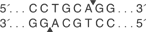
\includegraphics[scale=.5]{Sbf-I-cutsite_1_v1_000015}} }
\newglossaryentry{SbfI}{name=SbfI, description={restriction enzyme with the recognition sequence CCTGCA$\downarrow$GG} }
\newglossaryentry{XhoI}{name=XhoI, description={restriction enzyme with the recognition sequence C$\downarrow$TCGAG} }
\newglossaryentry{heterochromatin}{name=heterochromatin, description={Chromatin that remains in a highly condensed state throughout the cell cycle}}
\newglossaryentry{contig}{name=contig, description={longer consensus sequence derived from assembling smaller overlapping sequence reads}}
\newglossaryentry{linked RAD tag site}{name=linked RAD tag site, description={position in the reference sequence with at least one \gls{concordant} read pair on each side of a putative restriction site and the SE reads overlapping each other as expected from the restriction enzyme}}
\newglossaryentry{proper pair}{name=proper pair, description={read pair from illumina paired-end sequencing that got mapped to a reference in the correct orientation within a maximum expected distance from each other that is determined by the fragment size selection during the sequencing library preparation. Also called a \gls{concordant}ly mapping pair}}
\newglossaryentry{kmer}{name=kmer, description={subsequence with a specified length (k) of a longer sequence}}
\newglossaryentry{e-value}{name=Expect (E) value, description={The Expect value (E) is a parameter that describes the number of hits one can "expect" to see by chance when searching a database of a particular size}}
\newglossaryentry{read}{name=read, description={any sequence that comes out of the sequencer}}
\newglossaryentry{edit distance}{name=edit distance, description={minimum number of operations (one symbol insertion, deletion or substitution) required to change one string of symbols into another. Also known as \emph{Levenshtein distance}}}
\newglossaryentry{Ct}{name={C$_{t}$}, description={PCR cycle when a certain fluorescent threshold is reached}}
\newglossaryentry{mqs}{name={mapping quality score}, description={The mapping quality score \emph{Q} is the Phred transformation of the estimate of the probability \emph{p} that the reported mapping position does not correspond to the read's true point of origin: $Q = -10 \log_{10} p$. The way \emph{p} is estimated is different for each mapping programme, but in any case a mapping quality score \emph{Q} of 3 roughly corresponds to a mis-mapping probability \emph{p} of 0.5, i. e. the read has an estimated 50\% chance to have derived from a location other than the one reported}}
\newglossaryentry{discordant}{name=discordant, description={A read pair is called discordant if it aligns without the expected relative mate orientation (here: forward--reverse or reverse--forward) or outside the expected range of distances between mates. Note that \texttt{bowtie2} only calls discordant read pair mappings if both reads map \emph{uniquely}. Here, I am NOT adopting this requirement}}
\newglossaryentry{concordant}{name=concordant, description={A read pair is called concordant if it aligns with the expected relative mate orientation (here: forward--reverse or reverse--forward) and within the expected range of distances between mates. This is also called a \gls{proper pair}. The complement of \gls{discordant}}}
\newglossaryentry{Levenshtein distance}{name=Levenshtein distance, description={The Levenshtein distance is equal to the minimum number of operations (edits) required to transform one string into another. The allowed operations are single character insertions, deletions and substitutions. This is also known as edit distance.}}
\newglossaryentry{all pairs}{name={all pairs}, description={all the pairs of sequences below a given Levenshtein distance are identified during the graph construction phase}}
\newglossaryentry{transitive clusters}{name=transitive clusters, description={Two read clusters are merged if the distance of any pair of reads between the clusters is below threshold. After merging, the newly created cluster can contain read pairs with distance above the clustering threshold}}
\newglossaryentry{graph}{name=graph, description={A network of connected sequences. Two sequences are directly connected if they match with distance below a threshold. The distance is a measure of the strength of connection, aka "edge weight". Graphs can be stored as a list of pairs of sequences, with an optional edge weight. All graphs here should be "undirected cyclic graphs"}}
\newglossaryentry{Nmer}{name=\emph{N}mer, description={synonymous to kmer, unit, word; a subsequence of size \emph{N} that is overlapping or contiguous with the next subsequence of size \emph{N} and stored in a dictionnary (aka hash) for fast lookup}}
\newglossaryentry{population allele frequency}{name=population allele frequency, description={The population allele frequency is the (unknown) frequency of the allele in the entire population}}
\newglossaryentry{sample allele frequency}{name=sample allele frequency, description={The sample allele frequency is the frequency of the allele among the individuals in a specific sample}}
\newglossaryentry{connected component}{name=connected component, description={All nodes (here sequence reads) after all--pairs search (and before clustering!) that are directly connected by an edge or indirectly connected via several nodes belong to the same connected component} }

%----------------
% Acronyms
%----------------
\newacronym{snp}{SNP}{single nucleotide polymorphism}
\newacronym{rad}{RAD}{Restriction Site associated DNA}
\newacronym{pe}{PE}{paired-end}
\newacronym{se}{SE}{single-end}
\newacronym{bp}{bp}{base pair}
\newacronym{Mbp}{Mbp}{mega base pairs}
\newacronym{Gbp}{Gbp}{giga base pairs}
\newacronym{indel}{indel}{small sequence insertion or deletion polymorphism}
\newacronym{SAM}{SAM}{Sequence Alignment/Map format}
\newacronym{EST}{EST}{expressed sequence tag}
\newacronym{ddRAD}{ddRAD}{double digest RAD}
\newacronym{ML}{ML}{maximum likelihood}
\newacronym{SFS}{SFS}{site frequency spectrum}
\newacronym{HWE}{HWE}{Hardy Weinberg equilibrium}
\newacronym{CI}{CI}{confidence interval}
\newacronym{EM}{EM}{Expectation Maximisation}
\newacronym{DEM}{DEM}{digital elevation model}
%\usepackage[toc]{glossaries}
%\renewcommand*{\glstextformat}[1]{\textsf{#1}}
%
%\newglossaryentry{fragment}{name=fragment, description={not a PCR duplicate}}
%
%\newacronym{snp}{SNP}{single nucleotide polymorphism}

%% ******************************** SVG *************************************
%\newcommand{\executeiffilenewer}[3]{%
%	\ifnum\pdfstrcmp{\pdffilemoddate{#1}}%
%	{\pdffilemoddate{#2}}>0%
%	{\immediate\write18{#3}}\fi%
%}
%\newcommand{\includesvg}[1]{%
%	\executeiffilenewer{#1.svg}{#1.pdf}%
%	{./inkscape -z -D -f #1.svg %
%	--export-pdf=#1.pdf --export-latex}%
%	\import{./Figs/Inkscape_Graphics}{#1.pdf_tex}%
%}



% ************************ Thesis Information & Meta-data **********************
% Thesis title and author information, reference file for biblatex
% ************************ Thesis Information & Meta-data **********************
%% The title of the thesis
\title{Writing your PhD thesis in \texorpdfstring{\\ \LaTeX2e}{LaTeX2e}}
%\texorpdfstring is used for PDF metadata. Usage:
%\texorpdfstring{LaTeX_Version}{PDF Version (non-latex)} eg.,
%\texorpdfstring{$sigma$}{sigma}

%% Subtitle (Optional)
\subtitle{Using the CUED template}

%% The full name of the author
\author{Krishna Kumar}

%% Department (eg. Department of Engineering, Maths, Physics)
\dept{Department of Engineering}

%% University and Crest
\university{University of Cambridge}
\crest{
\includegraphics[width=0.25\textwidth]{tuoslogo_key_cmyk_hi}}

%% You can redefine the submission text:
% Default as per the University guidelines:
% ``This dissertation is submitted for the degree of''
%\renewcommand{\submissiontext}{change the default text here if needed}

%% Full title of the Degree
\degreetitle{Doctor of Philosophy}

%% College affiliation (optional)
\college{King's College}

%% Submission date
% Default is set as {\monthname[\the\month]\space\the\year}
%\degreedate{September 2014} 

%% Meta information
\subject{LaTeX} \keywords{{LaTeX} {PhD Thesis} {Engineering} {University of
Cambridge}}


% ***************************** Abstract Separate ******************************
% To printout only the titlepage and the abstract with the PhD title and the
% author name for submission to the Student Registry, use the `abstract' option in
% the document class.

\ifdefineAbstract
 \pagestyle{empty}
 \includeonly{Declaration/declaration, Abstract/abstract}
\fi

% ***************************** Chapter Mode ***********************************
% The chapter mode allows user to only print particular chapters with references
% Title, Contents, Frontmatter are disabled by default
% Useful option to review a particular chapter or to send it to a supervisor.
% To use choose `chapter' option in the document class

\ifdefineChapter
 \includeonly{Chapter3/chapter3}
\fi

% ******************************** Front Matter ********************************
\IfFileExists{upquote.sty}{\usepackage{upquote}}{}
\begin{document}

%%%%%% -- KNITR SETUP -- %%%%%%%%%%%%%%%%%%%%

%%%%%%%%%%%%%%%%%%%%%%%%%%%%%%%%%%%%

\frontmatter

\begin{titlepage}
  \maketitle
\end{titlepage}


% ******************************* Thesis Dedidcation ********************************

\begin{dedication} 

I would like to dedicate this thesis to my grandmother who has never stopped believing in me.

\end{dedication}


\include{Declaration/declaration}
% ************************** Thesis Acknowledgements **************************

\begin{acknowledgements}      


And I would like to acknowledge Stefan Prost, Simon Baxter, John Davey, Toni Gossmann and G\"{u}nter K\"{o}hler. I am particularly grateful to Martina Ottenbruch for being my host during the last six months.


\end{acknowledgements}

% ************************** Thesis Abstract *****************************
% Use `abstract' as an option in the document class to print only the titlepage and the abstract.
\begin{abstract}
\gls{rad} is a molecular method involving restriction digestion and high throughput DNA sequencing. It promises the systematic subsampling of the genome and highly repeatable scoring of genetic variation in hundreds of individuals at current sequencing costs. However, it comes with its own problems. De novo assembly of \gls{rad} sequence data usually creates many putative reference tags that are only found in one or a few individuals leaving only relatively few markers for population genomic analyses. I here investigate three potential reasons for this outcome -- incomplete digestion, genomic religation and insufficient DNA template amount -- by looking at the occurrence of restriction enzyme recognition sequences within the resultant sequencing data of two different types of \gls{rad} libraries. 

Analysis of sequence clusters as well as the proportion of concordantly mapping read pairs against a \textit{Locusta} reference sequence suggest that incomplete digestion has affected one of the restriction enzymes used and thereby the amount of loci that could be sequenced at sufficient coverage across individuals. The other restriction enzyme is found to be much less affected by incomplete digestion and instead random religation of restriction fragments indicates an inefficient adapter ligation step that also leads to low read coverage across individuals. Finally, qPCR and read mapping against four newly reconstructed \gls{pe} contig pair reference sequences suggests that low amount of starting DNA and/or high loss of DNA during the library preparation are a major cause for the locus drop out observed in the de novo assembled read data.

In the second part of this thesis I am using \gls{rad} sequence data to make inferences about several aspects of the demographic history of two grasshopper subspecies. Sequence data was generated from 36 individuals sampled at the two opposite ends of a hybrid zone of two grasshopper subspecies that is characterised by hybrid male sterility. I use a state--of--the--art de novo assembly strategy that utilises the shotgun--type \gls{pe} reads from standard \gls{rad} to distinguish alleles from paralogs. I then conduct several population genomic analyses with the programme \texttt{ANGSD} that incorporates uncertainty in genotypes by using genotype likelihoods instead of called genotypes. Results based on more than 1 million filtered sites show the strong genetic differentiation of the two subspecies and a surprisingly high genetic diversity in the subspecies that is thought to be derived from a very distant glacial refuge. Further analysis of this data set promises to yield more insights.
\end{abstract}


% *********************** Adding TOC and List of Figures ***********************

\tableofcontents

\listoffigures

\listoftables

% \printnomencl[space] space can be set as 2em between symbol and description
%\printnomencl[3em]

\printnomencl

\printglossaries

% ******************************** Main Matter *********************************
\mainmatter

%%*******************************************************************************
%*********************************** First Chapter *****************************
%*******************************************************************************

\chapter{Getting started}  %Title of the First Chapter

\ifpdf
    \graphicspath{{Chapter1/Figs/Raster/}{Chapter1/Figs/PDF/}{Chapter1/Figs/}}
\else
    \graphicspath{{Chapter1/Figs/Vector/}{Chapter1/Figs/}}
\fi


%********************************** %First Section  **************************************
\section{What is loren ipsum? Title with math \texorpdfstring{$\sigma$}{[sigma]}} %Section - 1.1 

Lorem Ipsum is simply dummy text of the printing and typesetting industry (see 
Section~\ref{section1.3}). Lorem Ipsum~\citep{Aup91} has been the industry's 
standard dummy text ever since the 1500s, when an unknown printer took a galley 
of type and scrambled it to make a type specimen book. It has survived not only 
five centuries, but also the leap into electronic typesetting, remaining 
essentially unchanged. It was popularised in the 1960s with the release of 
Letraset sheets containing Lorem Ipsum passages, and more recently with desktop 
publishing software like Aldus PageMaker including versions of Lorem 
Ipsum~\citep{AAB95,Con90,LM65}.

The most famous equation in the world: $E^2 = (m_0c^2)^2 + (pc)^2$, which is 
known as the \textbf{energy-mass-momentum} relation as an in-line equation.

A {\em \LaTeX{} class file}\index{\LaTeX{} class file@LaTeX class file} is a file, which holds style information for a particular \LaTeX{}.


\begin{align}
CIF: \hspace*{5mm}F_0^j(a) = \frac{1}{2\pi \iota} \oint_{\gamma} \frac{F_0^j(z)}{z - a} dz
\end{align}

\nomenclature[z-cif]{$CIF$}{Cauchy's Integral Formula}                                % first letter Z is for Acronyms 
\nomenclature[a-F]{$F$}{complex function}                                                   % first letter A is for Roman symbols
\nomenclature[g-p]{$\pi$}{ $\simeq 3.14\ldots$}                                             % first letter G is for Greek Symbols
\nomenclature[g-i]{$\iota$}{unit imaginary number $\sqrt{-1}$}                      % first letter G is for Greek Symbols
\nomenclature[g-g]{$\gamma$}{a simply closed curve on a complex plane}  % first letter G is for Greek Symbols
\nomenclature[x-i]{$\oint_\gamma$}{integration around a curve $\gamma$} % first letter X is for Other Symbols
\nomenclature[r-j]{$j$}{superscript index}                                                       % first letter R is for superscripts
\nomenclature[s-0]{$0$}{subscript index}                                                        % first letter S is for subscripts


%********************************** %Second Section  *************************************
\section{Why do we use loren ipsum?} %Section - 1.2


It is a long established fact that a reader will be distracted by the readable content of a page when looking at its layout. The point of using Lorem Ipsum is that it has a more-or-less normal distribution of letters, as opposed to using `Content here, content here', making it look like readable English. Many desktop publishing packages and web page editors now use Lorem Ipsum as their default model text, and a search for `lorem ipsum' will uncover many web sites still in their infancy. Various versions have evolved over the years, sometimes by accident, sometimes on purpose (injected humour and the like).

%********************************** % Third Section  *************************************
\section{Where does it come from?}  %Section - 1.3 
\label{section1.3}

Contrary to popular belief, Lorem Ipsum is not simply random text. It has roots in a piece of classical Latin literature from 45 BC, making it over 2000 years old. Richard McClintock, a Latin professor at Hampden-Sydney College in Virginia, looked up one of the more obscure Latin words, consectetur, from a Lorem Ipsum passage, and going through the cites of the word in classical literature, discovered the undoubtable source. Lorem Ipsum comes from sections 1.10.32 and 1.10.33 of "de Finibus Bonorum et Malorum" (The Extremes of Good and Evil) by Cicero, written in 45 BC. This book is a treatise on the theory of ethics, very popular during the Renaissance. The first line of Lorem Ipsum, "Lorem ipsum dolor sit amet..", comes from a line in section 1.10.32.

The standard chunk of Lorem Ipsum used since the 1500s is reproduced below for those interested. Sections 1.10.32 and 1.10.33 from ``de Finibus Bonorum et Malorum" by Cicero are also reproduced in their exact original form, accompanied by English versions from the 1914 translation by H. Rackham

``Lorem ipsum dolor sit amet, consectetur adipisicing elit, sed do eiusmod tempor incididunt ut labore et dolore magna aliqua. Ut enim ad minim veniam, quis nostrud exercitation ullamco laboris nisi ut aliquip ex ea commodo consequat. Duis aute irure dolor in reprehenderit in voluptate velit esse cillum dolore eu fugiat nulla pariatur. Excepteur sint occaecat cupidatat non proident, sunt in culpa qui officia deserunt mollit anim id est laborum."

Section 1.10.32 of ``de Finibus Bonorum et Malorum", written by Cicero in 45 BC: ``Sed ut perspiciatis unde omnis iste natus error sit voluptatem accusantium doloremque laudantium, totam rem aperiam, eaque ipsa quae ab illo inventore veritatis et quasi architecto beatae vitae dicta sunt explicabo. Nemo enim ipsam voluptatem quia voluptas sit aspernatur aut odit aut fugit, sed quia consequuntur magni dolores eos qui ratione voluptatem sequi nesciunt. Neque porro quisquam est, qui dolorem ipsum quia dolor sit amet, consectetur, adipisci velit, sed quia non numquam eius modi tempora incidunt ut labore et dolore magnam aliquam quaerat voluptatem. Ut enim ad minima veniam, quis nostrum exercitationem ullam corporis suscipit laboriosam, nisi ut aliquid ex ea commodi consequatur? Quis autem vel eum iure reprehenderit qui in ea voluptate velit esse quam nihil molestiae consequatur, vel illum qui dolorem eum fugiat quo voluptas nulla pariatur?"

1914 translation by H. Rackham: ``But I must explain to you how all this mistaken idea of denouncing pleasure and praising pain was born and I will give you a complete account of the system, and expound the actual teachings of the great explorer of the truth, the master-builder of human happiness. No one rejects, dislikes, or avoids pleasure itself, because it is pleasure, but because those who do not know how to pursue pleasure rationally encounter consequences that are extremely painful. Nor again is there anyone who loves or pursues or desires to obtain pain of itself, because it is pain, but because occasionally circumstances occur in which toil and pain can procure him some great pleasure. To take a trivial example, which of us ever undertakes laborious physical exercise, except to obtain some advantage from it? But who has any right to find fault with a man who chooses to enjoy a pleasure that has no annoying consequences, or one who avoids a pain that produces no resultant pleasure?"

Section 1.10.33 of ``de Finibus Bonorum et Malorum", written by Cicero in 45 BC: ``At vero eos et accusamus et iusto odio dignissimos ducimus qui blanditiis praesentium voluptatum deleniti atque corrupti quos dolores et quas molestias excepturi sint occaecati cupiditate non provident, similique sunt in culpa qui officia deserunt mollitia animi, id est laborum et dolorum fuga. Et harum quidem rerum facilis est et expedita distinctio. Nam libero tempore, cum soluta nobis est eligendi optio cumque nihil impedit quo minus id quod maxime placeat facere possimus, omnis voluptas assumenda est, omnis dolor repellendus. Temporibus autem quibusdam et aut officiis debitis aut rerum necessitatibus saepe eveniet ut et voluptates repudiandae sint et molestiae non recusandae. Itaque earum rerum hic tenetur a sapiente delectus, ut aut reiciendis voluptatibus maiores alias consequatur aut perferendis doloribus asperiores repellat."

1914 translation by H. Rackham: ``On the other hand, we denounce with righteous indignation and dislike men who are so beguiled and demoralized by the charms of pleasure of the moment, so blinded by desire, that they cannot foresee the pain and trouble that are bound to ensue; and equal blame belongs to those who fail in their duty through weakness of will, which is the same as saying through shrinking from toil and pain. These cases are perfectly simple and easy to distinguish. In a free hour, when our power of choice is untrammelled and when nothing prevents our being able to do what we like best, every pleasure is to be welcomed and every pain avoided. But in certain circumstances and owing to the claims of duty or the obligations of business it will frequently occur that pleasures have to be repudiated and annoyances accepted. The wise man therefore always holds in these matters to this principle of selection: he rejects pleasures to secure other greater pleasures, or else he endures pains to avoid worse pains."

%\include{Chapter2/chapter2}
%
\documentclass[a4paper,12pt,times,numbered,print,index]{PhDThesisPSnPDF}
\usepackage[]{graphicx}\usepackage[]{color}
%% maxwidth is the original width if it is less than linewidth
%% otherwise use linewidth (to make sure the graphics do not exceed the margin)
\makeatletter
\def\maxwidth{ %
  \ifdim\Gin@nat@width>\linewidth
    \linewidth
  \else
    \Gin@nat@width
  \fi
}
\makeatother

\definecolor{fgcolor}{rgb}{0.345, 0.345, 0.345}
\newcommand{\hlnum}[1]{\textcolor[rgb]{0.686,0.059,0.569}{#1}}%
\newcommand{\hlstr}[1]{\textcolor[rgb]{0.192,0.494,0.8}{#1}}%
\newcommand{\hlcom}[1]{\textcolor[rgb]{0.678,0.584,0.686}{\textit{#1}}}%
\newcommand{\hlopt}[1]{\textcolor[rgb]{0,0,0}{#1}}%
\newcommand{\hlstd}[1]{\textcolor[rgb]{0.345,0.345,0.345}{#1}}%
\newcommand{\hlkwa}[1]{\textcolor[rgb]{0.161,0.373,0.58}{\textbf{#1}}}%
\newcommand{\hlkwb}[1]{\textcolor[rgb]{0.69,0.353,0.396}{#1}}%
\newcommand{\hlkwc}[1]{\textcolor[rgb]{0.333,0.667,0.333}{#1}}%
\newcommand{\hlkwd}[1]{\textcolor[rgb]{0.737,0.353,0.396}{\textbf{#1}}}%

\usepackage{framed}
\makeatletter
\newenvironment{kframe}{%
 \def\at@end@of@kframe{}%
 \ifinner\ifhmode%
  \def\at@end@of@kframe{\end{minipage}}%
  \begin{minipage}{\columnwidth}%
 \fi\fi%
 \def\FrameCommand##1{\hskip\@totalleftmargin \hskip-\fboxsep
 \colorbox{shadecolor}{##1}\hskip-\fboxsep
     % There is no \\@totalrightmargin, so:
     \hskip-\linewidth \hskip-\@totalleftmargin \hskip\columnwidth}%
 \MakeFramed {\advance\hsize-\width
   \@totalleftmargin\z@ \linewidth\hsize
   \@setminipage}}%
 {\par\unskip\endMakeFramed%
 \at@end@of@kframe}
\makeatother

\definecolor{shadecolor}{rgb}{.97, .97, .97}
\definecolor{messagecolor}{rgb}{0, 0, 0}
\definecolor{warningcolor}{rgb}{1, 0, 1}
\definecolor{errorcolor}{rgb}{1, 0, 0}
\newenvironment{knitrout}{}{} % an empty environment to be redefined in TeX

\usepackage{alltt}
\newcommand{\SweaveOpts}[1]{}  % do not interfere with LaTeX
\newcommand{\SweaveInput}[1]{} % because they are not real TeX commands
\newcommand{\Sexpr}[1]{}       % will only be parsed by R



% ******************************************************************************
% ******************************* Class Options ********************************
% *********************** See README for more details **************************
% ******************************************************************************

% `a4paper'(The University of Cambridge PhD thesis guidelines recommends a page
% size a4 - default option) or `a5paper': A5 Paper size is also allowed as per
% the Cambridge University Engineering Deparment guidelines for PhD thesis
%
% `11pt' or `12pt'(default): Font Size 10pt is NOT recommended by the University
% guidelines
%
% `oneside' or `twoside'(default): Printing double side (twoside) or single
% side.
%
% `print': Use `print' for print version with appropriate margins and page
% layout. Leaving the options field blank will activate Online version.
%
% `index': For index at the end of the thesis
%
% `draft': For draft mode without loading any images (same as draft in book)
%
% `draftmode': Special draft mode with line numbers, images, and water mark with
% timestamp and custom text. Position of the text can also be modified.
%
% `abstract': To generate only the title page and abstract page with
% dissertation title and name, to submit to the Student Registry
%
% `chapter`: This option enables only the specified chapter and it's references
%  Useful for review and corrections.
%
% ************************* Custom Page Margins ********************************
%
% `custommargin`: Use `custommargin' in options to activate custom page margins,
% which can be defined in the preamble.tex. Custom margin will override
% print/online margin setup.
%
% *********************** Choosing the Fonts in Class Options ******************
%
% `times' : Times font with math support. (The Cambridge University guidelines
% recommend using times)
%
% `fourier': Utopia Font with Fourier Math font (Font has to be installed)
%            It's a free font.
%
% `customfont': Use `customfont' option in the document class and load the
% package in the preamble.tex
%
% default or leave empty: `Latin Modern' font will be loaded.
%
% ********************** Choosing the Bibliography style ***********************
%
% `authoryear': For author-year citation eg., Krishna (2013)
%
% `numbered': (Default Option) For numbered and sorted citation e.g., [1,5,2]
%
% `custombib': Define your own bibliography style in the `preamble.tex' file.
%              `\RequirePackage[square, sort, numbers, authoryear]{natbib}'.
%              This can be also used to load biblatex instead of natbib
%              (See Preamble)
%
% **************************** Choosing the Page Style *************************
%
% `default (leave empty)': For Page Numbers in Header (Left Even, Right Odd) and
% Chapter Name in Header (Right Even) and Section Name (Left Odd). Blank Footer.
%
% `PageStyleI': Chapter Name next & Page Number on Even Side (Left Even).
% Section Name & Page Number in Header on Odd Side (Right Odd). Footer is empty.
%
% `PageStyleII': Chapter Name on Even Side (Left Even) in Header. Section Number
% and Section Name in Header on Odd Side (Right Odd). Page numbering in footer


% ********************************** Preamble **********************************
% Preamble: Contains packages and user-defined commands and settings
% ******************************************************************************
% ****************************** Custom Margin *********************************

% Add `custommargin' in the document class options to use this section
% Set {innerside margin / outerside margin / topmargin / bottom margin}  and
% other page dimensions
\ifsetCustomMargin
  \RequirePackage[left=42mm,right=35mm,top=25mm,bottom=20mm]{geometry}
  \setFancyHdr % To apply fancy header after geometry package is loaded
\fi

% *****************************************************************************
% ******************* Fonts (like different typewriter fonts etc.)*************

% Add `customfont' in the document class option to use this section

\ifsetCustomFont
  % Set your custom font here and use `customfont' in options. Leave empty to
  % load computer modern font (default LaTeX font).
  \RequirePackage{helvet}
\fi

% *****************************************************************************
% **************************** Custom Packages ********************************
\usepackage{import}

%\usepackage{comment}

\usepackage{epigraph}

%% ---- package for formatting code with line numbers
\usepackage{fancyvrb} %% for verbatim text

\usepackage{ulem} % more underlining and other font effects

% ************************** Custom Floats **********************************
\usepackage{float}
\floatstyle{ruled}
\newfloat{cmd}{htb}{loc}[chapter]
\floatname{cmd}{Command}
% **** **** **** **** **** **** **** ****

%% ---- provides "\rowcolors" command
\usepackage[dvipsnames,table]{xcolor}

\usepackage{subcaption}

% ---- the following package call ensures that floats will not pass a section boundary ----
\usepackage[section]{placeins}
% ---- insert “\FloatBarrier” at places that floats should not move past, perhaps at every “\section”.

% ---- if I want to extract LaTeX formulas, for instance, 
% ---- to convert them into other picture formats from pdf
%\usepackage[active,tightpage]{preview}
% ---- use \begin{preiview} ... \end{preview}

\usepackage{relsize}
\renewcommand\RSsmallest{4pt}

%------ the following package can be used for Word Review function mimicking comments ----------%
\usepackage[textsize=tiny, textwidth=3cm, color=Dandelion, colorinlistoftodos]{todonotes} % specify ``disable'' to turn off all notes
\newcommand{\addcit}[1]{\todo[color=yellow!90,nolist]{#1}}
\newcommand{\comment}[1]{\todo[color=green!40,noline,nolist]{#1}} % the "comment" package also defines a command "\comment", so cannot use both
\newcommand{\longcomment}[1]{\todo[color=green!40,inline,nolist]{#1}}
\newcommand{\roger}[1]{\todo[color=blue!40]{Roger:\newline{}#1}}

%\ifsetDraft
%	\usepackage[textsize=tiny, textwidth=3cm, color=Dandelion, colorinlistoftodos]{todonotes} % specify ``disable'' to turn off all notes
%	\newcommand{\addcit}[1]{\todo[color=yellow!90,nolist]{#1}}
%	\newcommand{\comment}[1]{\todo[color=green!40,noline,nolist]{#1}}
%	\newcommand{\longcomment}[1]{\todo[color=green!40,inline,nolist]{#1}}
%	\newcommand{\roger}[1]{\todo[color=blue!40]{Roger:\newline{}#1}}
%\else
%	\newcommand{\addcit}[1]{}
%	\newcommand{\comment}[1]{}
%	\newcommand{\longcomment}[1]{}
%	\newcommand{\roger}[1]{}
%	\newcommand{\listoftodos}{}
%	\newcommand{\todo}{}
%\fi

%\usepackage{setspace}
%\newcommand{\note}[2][] {\todo[caption={#2}, #1] {\begin{spacing}{0.8}#2\end{spacing}}}

\usepackage{pdflscape}
\usepackage{lscape} % offers landscape environment, \begin{landscape}

% ---- for verbatim in captions. Usage: \cprotect\caption{...} ----
\usepackage{cprotect} 


% ************************* Algorithms and Pseudocode **************************

%\usepackage{algpseudocode}


% ********************Captions and Hyperreferencing / URL **********************

% Captions: This makes captions of figures use a boldfaced small font.
%\RequirePackage[small,bf]{caption}

\RequirePackage[labelsep=space,font=small,labelfont=bf,tableposition=top]{caption}
\DeclareCaptionLabelFormat{continued}{#1 #2 continued} 
\captionsetup[ContinuedFloat]{labelformat=continued}
\renewcommand{\figurename}{Fig.} %to support older versions of captions.sty
\usepackage{varioref}

\hypersetup{%
colorlinks=true,% 
citecolor=black,% 
linkcolor=black,
urlcolor=black% 
}



% *************************** Graphics and figures *****************************

%\usepackage{subfigure}

%\usepackage{rotating}
%\usepackage{wrapfig}

% Uncomment the following two lines to force Latex to place the figure.
% Use [H] when including graphics. Note 'H' instead of 'h'
%\usepackage{float}
%\restylefloat{figure}

% Subcaption package is also available in the sty folder you can use that by
% uncommenting the following line
% This is for people stuck with older versions of texlive
%\usepackage{sty/caption/subcaption}
\usepackage{subcaption}

% ********************************** Tables ************************************
\usepackage{booktabs} % For professional looking tables
\usepackage{multirow}
\usepackage{ctable}
\usepackage{colortbl}

%\usepackage{multicol}
%\usepackage{longtable}
%\usepackage{tabularx}


% ***************************** Math and SI Units ******************************

\usepackage{amsfonts}
\usepackage{amsmath}
\usepackage{amssymb}
\usepackage{siunitx} % use this package module for SI units


% ******************************* Line Spacing *********************************

% Choose linespacing as appropriate. Default is one-half line spacing as per the
% University guidelines

%\usepackage{setspace} % already loaded
% \doublespacing
% \onehalfspacing
% \singlespacing
% \setstretch{<baselinestretch>}

% e. g.:
%\begin{spacing}{1.2}
%\tableofcontents
%\listoffigures
%\listoftables
%\end{spacing}
\raggedbottom % leaves empty space at the bottom of pages if necessary


% ************************ Formatting / Footnote *******************************

% Don't break enumeration (etc.) across pages in an ugly manner (default 10000)
%\clubpenalty=500
%\widowpenalty=500

%\usepackage[perpage]{footmisc} %Range of footnote options

\renewcommand{\paragraph}[1]{ \textsc{#1} }


% *****************************************************************************
% *************************** Bibliography  and References ********************

%\usepackage{cleveref} %Referencing without need to explicitly state fig /table

% Add `custombib' in the document class option to use this section
\ifuseCustomBib
   \RequirePackage[square, sort, numbers, authoryear]{natbib} % CustomBib

% If you would like to use biblatex for your reference management, as opposed to the default `natbibpackage` pass the option `custombib` in the document class. Comment out the previous line to make sure you don't load the natbib package. Uncomment the following lines and specify the location of references.bib file

%\RequirePackage[backend=biber, style=numeric-comp, citestyle=numeric, sorting=nty, natbib=true]{biblatex}
%\bibliography{References/references} %Location of references.bib only for biblatex

\fi

% changes the default name `Bibliography` -> `References'
\renewcommand{\bibname}{References}


% *****************************************************************************
% *************** Changing the Visual Style of Chapter Headings ***************
% This section on visual style is from https://github.com/cambridge/thesis

% Uncomment the section below. Requires titlesec package.

%\RequirePackage{titlesec}
%\newcommand{\PreContentTitleFormat}{\titleformat{\chapter}[display]{\scshape\Large}
%{\Large\filleft{\chaptertitlename} \Huge\thechapter}
%{1ex}{}
%[\vspace{1ex}\titlerule]}
%\newcommand{\ContentTitleFormat}{\titleformat{\chapter}[display]{\scshape\huge}
%{\Large\filleft{\chaptertitlename} \Huge\thechapter}{1ex}
%{\titlerule\vspace{1ex}\filright}
%[\vspace{1ex}\titlerule]}
%\newcommand{\PostContentTitleFormat}{\PreContentTitleFormat}
%\PreContentTitleFormat


% ******************************************************************************
% ************************* User Defined Commands ******************************
% ******************************************************************************

% *********** To change the name of Table of Contents / LOF and LOT ************

%\renewcommand{\contentsname}{My Table of Contents}
%\renewcommand{\listfigurename}{My List of Figures}
%\renewcommand{\listtablename}{My List of Tables}

\newcommand{\marginal}[1]{
	\leavevmode\marginpar{\tiny\raggedright#1\par}}


% ********************** TOC depth and numbering depth *************************

\setcounter{secnumdepth}{2}
\setcounter{tocdepth}{2}


% ******************************* Nomenclature *********************************
 
% To change the name of the Nomenclature section, uncomment the following line

%\renewcommand{\nomname}{Symbols}


% ********************************* Appendix ***********************************

% The default value of both \appendixtocname and \appendixpagename is `Appendices'. These names can all be changed via:

%\renewcommand{\appendixtocname}{List of appendices}
%\renewcommand{\appendixname}{Appndx}

% ******************************** Draft Mode **********************************

% Uncomment to disable figures in `draftmode'
%\setkeys{Gin}{draft=true}  % set draft to false to enable figures in `draft'

% These options are active only during the draft mode
% Default text is "Draft"
%\SetDraftText{DRAFT}

% Default Watermark location is top. Location (top/bottom)
%\SetDraftWMPosition{bottom}

% Draft Version - default is v1.0
%\SetDraftVersion{v1.1}

% Draft Text grayscale value (should be between 0-black and 1-white)
% Default value is 0.75
%\SetDraftGrayScale{0.8}


%% Todo notes functionality
%% Uncomment the following lines to have todonotes.

%\ifsetDraft
%	\usepackage[colorinlistoftodos]{todonotes}
%	\newcommand{\mynote}[1]{\todo[author=kks32,size=\small,inline,color=green!40]{#1}}
%\else
%	\newcommand{\mynote}[1]{}
%	\newcommand{\listoftodos}{}
%\fi

% Example todo: \mynote{Hey! I have a note}

%%******************************** Glossary ***************************************************
\usepackage[toc,acronym]{glossaries}

% suppress page number list in glossary:
%\usepackage[nonumberlist]{glossaries}
%% *** \usepackage[toc,acronym]{glossaries}
% suppress page number list in glossary:
%\usepackage[nonumberlist]{glossaries}

%
% -- put the following code into a .latexmkrc file in the directory from where you run Latexmk --
%
%# add glossary generation to LATEXMK routine
%# ==========================================
%# taken from:
%# http://tex.stackexchange.com/questions/1226/how-to-make-latexmk-use-makeglossaries
%
%add_cus_dep('glo', 'gls', 0, 'run_makeglossaries');
%add_cus_dep('acn', 'acr', 0, 'run_makeglossaries');
%
%sub run_makeglossaries {
%  if ( $silent ) {
%    system "makeglossaries -q $_[0]";
%  }
%  else {
%    system "makeglossaries $_[0]";
%  };
%}
%
%push @generated_exts, 'glo', 'gls', 'glg';
%push @generated_exts, 'acn', 'acr', 'alg';
%$clean_ext .= ' %R.ist %R.xdy';

\makeglossaries

\renewcommand*{\glstextformat}[1]{\textsf{#1}}
%\renewcommand*{\glshyperlink}[1]{\textsf{#1}}

%--------------
% Glossary
%--------------
\newglossaryentry{fragment}{name=fragment, description={not a PCR duplicate. With paired reads from standard RAD (i. e. including random shearing of restriction fragments) typically identified by having different PE read sequences or different insert sizes after read mapping against a reference}}
\newglossaryentry{RAD tag}{name=RAD tag, description={genetic marker from RAD sequencing; the sequence up or downstream of a restriction site}}
\newglossaryentry{barcode}{name=barcode, description={short DNA sequence incorporated into adapter oligonucleotides that becomes part of the sequence read. Barcodes are used in order to be able to pool the DNA of different individuals, populations, treatments, etc. into one library that can be sequenced on one lane of an illumina flow cell}}
\newglossaryentry{index}{name=index, description={similar to barcode and serves the same purpose; generally incorporated into the centre of the adapter so that special sequencing run for the index is required} }
%\newglossaryentry{SbfI}{name=SbfI, description={restriction enzyme with the recognition sequence 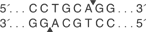
\includegraphics[scale=.5]{Sbf-I-cutsite_1_v1_000015}} }
\newglossaryentry{SbfI}{name=SbfI, description={restriction enzyme with the recognition sequence CCTGCA$\downarrow$GG} }
\newglossaryentry{XhoI}{name=XhoI, description={restriction enzyme with the recognition sequence C$\downarrow$TCGAG} }
\newglossaryentry{heterochromatin}{name=heterochromatin, description={Chromatin that remains in a highly condensed state throughout the cell cycle}}
\newglossaryentry{contig}{name=contig, description={longer consensus sequence derived from assembling smaller overlapping sequence reads}}
\newglossaryentry{linked RAD tag site}{name=linked RAD tag site, description={position in the reference sequence with at least one \gls{concordant} read pair on each side of a putative restriction site and the SE reads overlapping each other as expected from the restriction enzyme}}
\newglossaryentry{proper pair}{name=proper pair, description={read pair from illumina paired-end sequencing that got mapped to a reference in the correct orientation within a maximum expected distance from each other that is determined by the fragment size selection during the sequencing library preparation. Also called a \gls{concordant}ly mapping pair}}
\newglossaryentry{kmer}{name=kmer, description={subsequence with a specified length (k) of a longer sequence}}
\newglossaryentry{e-value}{name=Expect (E) value, description={The Expect value (E) is a parameter that describes the number of hits one can "expect" to see by chance when searching a database of a particular size}}
\newglossaryentry{read}{name=read, description={any sequence that comes out of the sequencer}}
\newglossaryentry{edit distance}{name=edit distance, description={minimum number of operations (one symbol insertion, deletion or substitution) required to change one string of symbols into another. Also known as \emph{Levenshtein distance}}}
\newglossaryentry{Ct}{name={C$_{t}$}, description={PCR cycle when a certain fluorescent threshold is reached}}
\newglossaryentry{mqs}{name={mapping quality score}, description={The mapping quality score \emph{Q} is the Phred transformation of the estimate of the probability \emph{p} that the reported mapping position does not correspond to the read's true point of origin: $Q = -10 \log_{10} p$. The way \emph{p} is estimated is different for each mapping programme, but in any case a mapping quality score \emph{Q} of 3 roughly corresponds to a mis-mapping probability \emph{p} of 0.5, i. e. the read has an estimated 50\% chance to have derived from a location other than the one reported}}
\newglossaryentry{discordant}{name=discordant, description={A read pair is called discordant if it aligns without the expected relative mate orientation (here: forward--reverse or reverse--forward) or outside the expected range of distances between mates. Note that \texttt{bowtie2} only calls discordant read pair mappings if both reads map \emph{uniquely}. Here, I am NOT adopting this requirement}}
\newglossaryentry{concordant}{name=concordant, description={A read pair is called concordant if it aligns with the expected relative mate orientation (here: forward--reverse or reverse--forward) and within the expected range of distances between mates. This is also called a \gls{proper pair}. The complement of \gls{discordant}}}
\newglossaryentry{Levenshtein distance}{name=Levenshtein distance, description={The Levenshtein distance is equal to the minimum number of operations (edits) required to transform one string into another. The allowed operations are single character insertions, deletions and substitutions. This is also known as edit distance.}}
\newglossaryentry{all pairs}{name={all pairs}, description={all the pairs of sequences below a given Levenshtein distance are identified during the graph construction phase}}
\newglossaryentry{transitive clusters}{name=transitive clusters, description={Two read clusters are merged if the distance of any pair of reads between the clusters is below threshold. After merging, the newly created cluster can contain read pairs with distance above the clustering threshold}}
\newglossaryentry{graph}{name=graph, description={A network of connected sequences. Two sequences are directly connected if they match with distance below a threshold. The distance is a measure of the strength of connection, aka "edge weight". Graphs can be stored as a list of pairs of sequences, with an optional edge weight. All graphs here should be "undirected cyclic graphs"}}
\newglossaryentry{Nmer}{name=\emph{N}mer, description={synonymous to kmer, unit, word; a subsequence of size \emph{N} that is overlapping or contiguous with the next subsequence of size \emph{N} and stored in a dictionnary (aka hash) for fast lookup}}
\newglossaryentry{population allele frequency}{name=population allele frequency, description={The population allele frequency is the (unknown) frequency of the allele in the entire population}}
\newglossaryentry{sample allele frequency}{name=sample allele frequency, description={The sample allele frequency is the frequency of the allele among the individuals in a specific sample}}
\newglossaryentry{connected component}{name=connected component, description={All nodes (here sequence reads) after all--pairs search (and before clustering!) that are directly connected by an edge or indirectly connected via several nodes belong to the same connected component} }

%----------------
% Acronyms
%----------------
\newacronym{snp}{SNP}{single nucleotide polymorphism}
\newacronym{rad}{RAD}{Restriction Site associated DNA}
\newacronym{pe}{PE}{paired-end}
\newacronym{se}{SE}{single-end}
\newacronym{bp}{bp}{base pair}
\newacronym{Mbp}{Mbp}{mega base pairs}
\newacronym{Gbp}{Gbp}{giga base pairs}
\newacronym{indel}{indel}{small sequence insertion or deletion polymorphism}
\newacronym{SAM}{SAM}{Sequence Alignment/Map format}
\newacronym{EST}{EST}{expressed sequence tag}
\newacronym{ddRAD}{ddRAD}{double digest RAD}
\newacronym{ML}{ML}{maximum likelihood}
\newacronym{SFS}{SFS}{site frequency spectrum}
\newacronym{HWE}{HWE}{Hardy Weinberg equilibrium}
\newacronym{CI}{CI}{confidence interval}
\newacronym{EM}{EM}{Expectation Maximisation}
\newacronym{DEM}{DEM}{digital elevation model}
%\usepackage[toc]{glossaries}
%\renewcommand*{\glstextformat}[1]{\textsf{#1}}
%
%\newglossaryentry{fragment}{name=fragment, description={not a PCR duplicate}}
%
%\newacronym{snp}{SNP}{single nucleotide polymorphism}

%% ******************************** SVG *************************************
%\newcommand{\executeiffilenewer}[3]{%
%	\ifnum\pdfstrcmp{\pdffilemoddate{#1}}%
%	{\pdffilemoddate{#2}}>0%
%	{\immediate\write18{#3}}\fi%
%}
%\newcommand{\includesvg}[1]{%
%	\executeiffilenewer{#1.svg}{#1.pdf}%
%	{./inkscape -z -D -f #1.svg %
%	--export-pdf=#1.pdf --export-latex}%
%	\import{./Figs/Inkscape_Graphics}{#1.pdf_tex}%
%}



% ************************ Thesis Information & Meta-data **********************
% Thesis title and author information, refernce file for biblatex
% ************************ Thesis Information & Meta-data **********************
%% The title of the thesis
\title{Writing your PhD thesis in \texorpdfstring{\\ \LaTeX2e}{LaTeX2e}}
%\texorpdfstring is used for PDF metadata. Usage:
%\texorpdfstring{LaTeX_Version}{PDF Version (non-latex)} eg.,
%\texorpdfstring{$sigma$}{sigma}

%% Subtitle (Optional)
\subtitle{Using the CUED template}

%% The full name of the author
\author{Krishna Kumar}

%% Department (eg. Department of Engineering, Maths, Physics)
\dept{Department of Engineering}

%% University and Crest
\university{University of Cambridge}
\crest{
\includegraphics[width=0.25\textwidth]{tuoslogo_key_cmyk_hi}}

%% You can redefine the submission text:
% Default as per the University guidelines:
% ``This dissertation is submitted for the degree of''
%\renewcommand{\submissiontext}{change the default text here if needed}

%% Full title of the Degree
\degreetitle{Doctor of Philosophy}

%% College affiliation (optional)
\college{King's College}

%% Submission date
% Default is set as {\monthname[\the\month]\space\the\year}
%\degreedate{September 2014} 

%% Meta information
\subject{LaTeX} \keywords{{LaTeX} {PhD Thesis} {Engineering} {University of
Cambridge}}


% ***************************** Abstract Separate ******************************
% To printout only the titlepage and the abstract with the PhD title and the
% author name for submission to the Student Registry, use the `abstract' option in
% the document class.

\ifdefineAbstract
 \pagestyle{empty}
 \includeonly{Declaration/declaration, Abstract/abstract}
\fi

% ***************************** Chapter Mode ***********************************
% The chapter mode allows user to only print particular chapters with references
% Title, Contents, Frontmatter are disabled by default
% Useful option to review a particular chapter or to send it to supervisior.
% To use choose `chapter' option in the document class

\ifdefineChapter
 \includeonly{Chapter3/chapter3}
\fi

% ******************************** Front Matter ********************************




\begin{document}
%%%%%% -- KNITR SETUP -- %%%%%%%%%%

%%%%%%%%%%%%%%%%%%%%%%%%%%

\chapter{My third chapter}

% **************************** Define Graphics Path **************************
\ifpdf
    \graphicspath{{Chapter3/Figs/Raster/}{Chapter3/Figs/PDF/}{Chapter3/Figs/}}
\else
    \graphicspath{{Chapter3/Figs/Vector/}{Chapter3/Figs/}}
\fi

\section{First section of the third chapter}
And now I begin my third chapter here \dots

And now to cite some more people~\citet{Rea85,Ancey1996}
\citet{Baird2008} were the first to publish about RAD.

\begin{figure}
\begin{knitrout}
\definecolor{shadecolor}{rgb}{0.969, 0.969, 0.969}\color{fgcolor}

{\centering 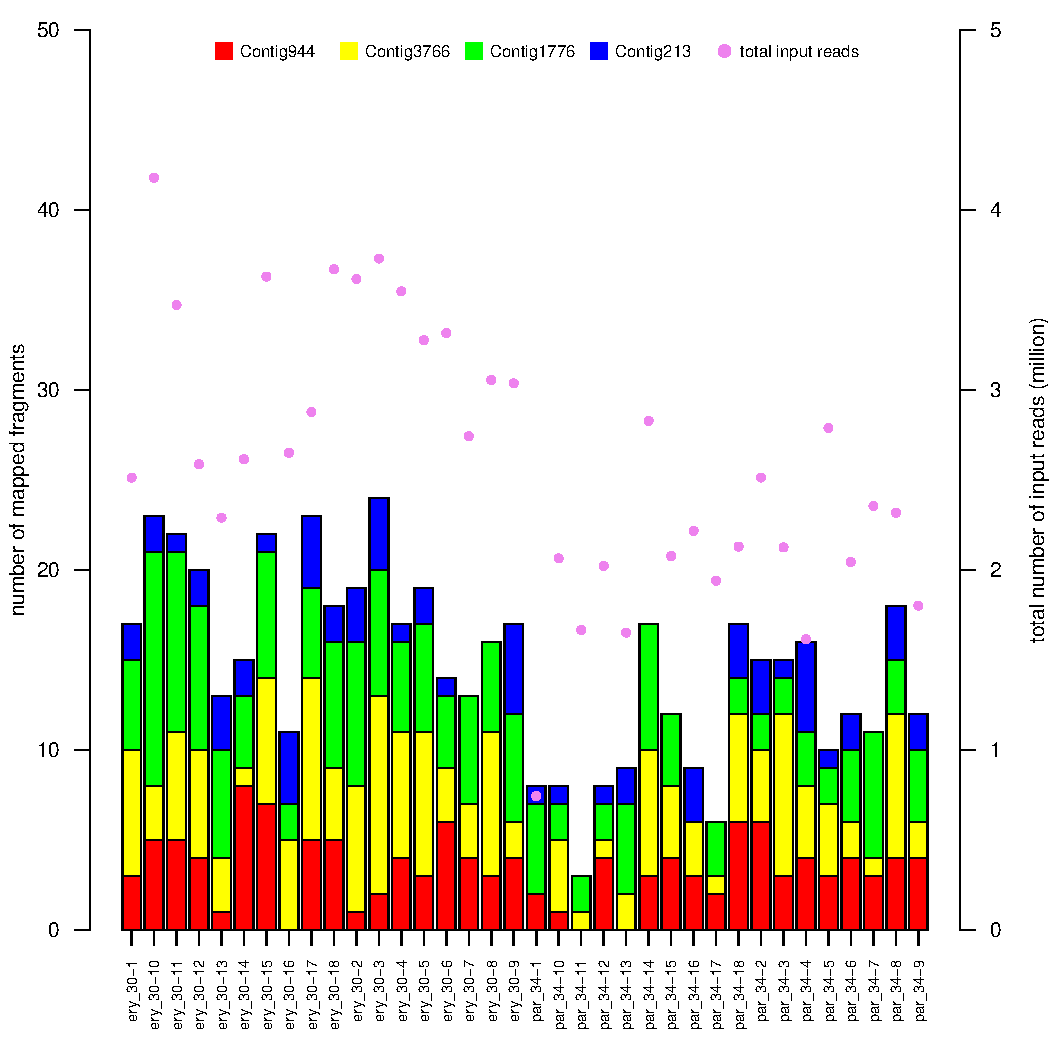
\includegraphics[width=\linewidth]{Chapter3/Figs/Knitr/fragments_mapped_per_ind-1} 

}



\end{knitrout}
\caption{Distribution of RAD fragment numbers mapped to 4 primer3ready reference contigs. A "fragment" is a properly mapped read pair from an individual with a unique insert size. If two read pairs on a RAD site from an individual have the same insert size, they constitute only one fragment, i. e. one read pair is likely to be a PCR duplicate.}
\label{fragments-mapped-per-ind}
\end{figure}


\subsection{First subsection in the first section}
\dots and some more 

\subsection{Second subsection in the first section}
\dots and some more \dots

\subsubsection{First subsub section in the second subsection}
\dots and some more in the first subsub section otherwise it all looks the same
doesn't it? well we can add some text to it \dots

\subsection{Third subsection in the first section}
\dots and some more \dots

\subsubsection{First subsub section in the third subsection}
\dots and some more in the first subsub section otherwise it all looks the same
doesn't it? well we can add some text to it and some more and some more and
some more and some more and some more and some more and some more \dots

\subsubsection{Second subsub section in the third subsection}
\dots and some more in the first subsub section otherwise it all looks the same
doesn't it? well we can add some text to it \dots

\section{Second section of the third chapter}
and here I write more \dots

\section{The layout of formal tables}
This section has been modified from ``Publication quality tables in \LaTeX*''
 by Simon Fear.

The layout of a table has been established over centuries of experience and 
should only be altered in extraordinary circumstances. 

When formatting a table, remember two simple guidelines at all times:

\begin{enumerate}
  \item Never, ever use vertical rules (lines).
  \item Never use double rules.
\end{enumerate}

These guidelines may seem extreme but I have
never found a good argument in favour of breaking them. For
example, if you feel that the information in the left half of
a table is so different from that on the right that it needs
to be separated by a vertical line, then you should use two
tables instead. Not everyone follows the second guideline:

There are three further guidelines worth mentioning here as they
are generally not known outside the circle of professional
typesetters and subeditors:

\begin{enumerate}\setcounter{enumi}{2}
  \item Put the units in the column heading (not in the body of
          the table).
  \item Always precede a decimal point by a digit; thus 0.1
      {\em not} just .1.
  \item Do not use `ditto' signs or any other such convention to
      repeat a previous value. In many circumstances a blank
      will serve just as well. If it won't, then repeat the value.
\end{enumerate}

A frequently seen mistake is to use `\textbackslash begin\{center\}' \dots `\textbackslash end\{center\}' inside a figure or table environment. This center environment can cause additional vertical space. If you want to avoid that just use `\textbackslash centering'


\begin{table}
\caption{A badly formatted table}
\centering
\label{table:bad_table}
\begin{tabular}{|l|c|c|c|c|}
\hline 
& \multicolumn{2}{c}{Species I} & \multicolumn{2}{c|}{Species II} \\ 
\hline
Dental measurement  & mean & SD  & mean & SD  \\ \hline 
\hline
I1MD & 6.23 & 0.91 & 5.2  & 0.7  \\
\hline 
I1LL & 7.48 & 0.56 & 8.7  & 0.71 \\
\hline 
I2MD & 3.99 & 0.63 & 4.22 & 0.54 \\
\hline 
I2LL & 6.81 & 0.02 & 6.66 & 0.01 \\
\hline 
CMD & 13.47 & 0.09 & 10.55 & 0.05 \\
\hline 
CBL & 11.88 & 0.05 & 13.11 & 0.04\\ 
\hline 
\end{tabular}
\end{table}

\begin{table}
\caption{A nice looking table}
\centering
\label{table:nice_table}
\begin{tabular}{l c c c c}
\hline 
\multirow{2}{*}{Dental measurement} & \multicolumn{2}{c}{Species I} & \multicolumn{2}{c}{Species II} \\ 
\cline{2-5}
  & mean & SD  & mean & SD  \\ 
\hline
I1MD & 6.23 & 0.91 & 5.2  & 0.7  \\

I1LL & 7.48 & 0.56 & 8.7  & 0.71 \\

I2MD & 3.99 & 0.63 & 4.22 & 0.54 \\

I2LL & 6.81 & 0.02 & 6.66 & 0.01 \\

CMD & 13.47 & 0.09 & 10.55 & 0.05 \\

CBL & 11.88 & 0.05 & 13.11 & 0.04\\ 
\hline 
\end{tabular}
\end{table}


\begin{table}
\caption{Even better looking table using booktabs}
\centering
\label{table:good_table}
\begin{tabular}{l c c c c}
\toprule
\multirow{2}{*}{Dental measurement} & \multicolumn{2}{c}{Species I} & \multicolumn{2}{c}{Species II} \\ 
\cmidrule{2-5}
  & mean & SD  & mean & SD  \\ 
\midrule
I1MD & 6.23 & 0.91 & 5.2  & 0.7  \\

I1LL & 7.48 & 0.56 & 8.7  & 0.71 \\

I2MD & 3.99 & 0.63 & 4.22 & 0.54 \\

I2LL & 6.81 & 0.02 & 6.66 & 0.01 \\

CMD & 13.47 & 0.09 & 10.55 & 0.05 \\

CBL & 11.88 & 0.05 & 13.11 & 0.04\\ 
\bottomrule
\end{tabular}
\end{table}
\bibliographystyle{elsarticle-harv} % use this to have URLs listed in References
\bibliography{References/Literature} % Path to your References.bib file
\end{document}

%\include{Chapter4/chapter4}
%\include{Chapter5/chapter5}
%\include{Chapter6/chapter6}
%\include{Chapter7/chapter7}


%%%%%% -- KNITR SETUP -- %%%%%%%%%%


%%%%%%%%%%%%%%%%%%%%%%%%%%

\chapter{My third chapter}

% **************************** Define Graphics Path **************************
\ifpdf
    \graphicspath{{Chapter3/Figs/Raster/}{Chapter3/Figs/PDF/}{Chapter3/Figs/}}
\else
    \graphicspath{{Chapter3/Figs/Vector/}{Chapter3/Figs/}}
\fi

% ************************************************************************************%   

\section{First section of the third chapter}
And now I begin my third chapter here \dots

And now to cite some more people~\citet{Rea85,Ancey1996}
\citet{Baird2008} were the first to publish about RAD. \SI{12,3}{\micro\metre}

Fig.~\vref{fragments-mapped-per-ind} shows the number of \glspl{fragment} mapped per individual.
I am trying to find \glspl{snp} among individuals of the sample.


\begin{figure}
\begin{knitrout}
\definecolor{shadecolor}{rgb}{0.969, 0.969, 0.969}\color{fgcolor}

{\centering 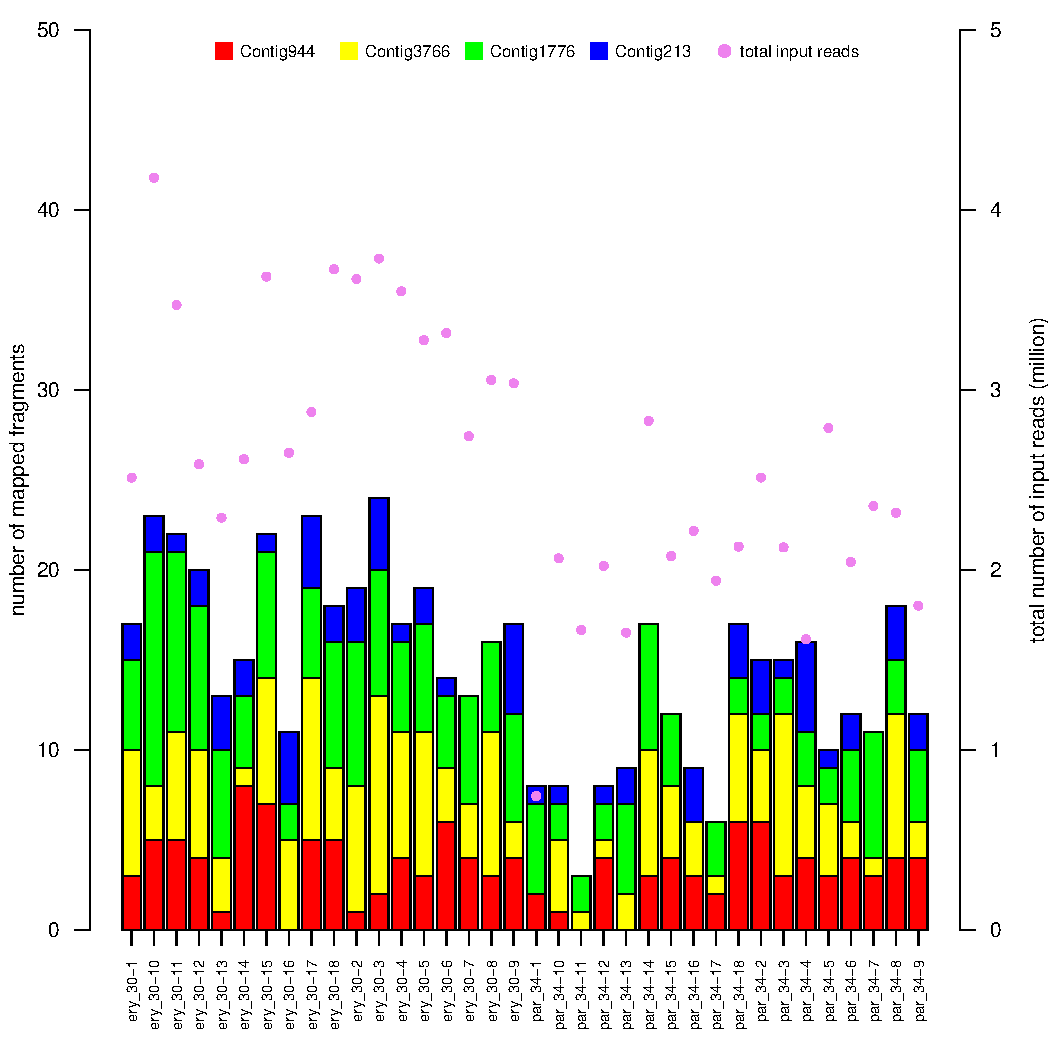
\includegraphics[width=\linewidth]{Chapter3/Figs/Knitr/fragments_mapped_per_ind-1} 

}



\end{knitrout}
\caption{Distribution of RAD fragment numbers mapped to 4 primer3ready reference contigs. 
A "fragment" is a properly mapped read pair from an individual with a unique insert size. 
If two read pairs on a RAD site from an individual have the same insert size, they constitute only one fragment, i. e. one read pair is likely to be a PCR duplicate.}
\label{fragments-mapped-per-ind}
\end{figure}

\begin{quote}
Bonzai: Are you as successful as you would like to be?

Zappa: I would say that the basic characteristic of my life is failure. 
If there is one thing that I excel at, it's failure -- I manage to fail at 100 percent of the things that I do. 
Since most of the things that I set out to do are theoretically impossible, it's very easy to fail. 
I've learned to live with it. 
In terms of machinery and personnel, there never seems to be enough to get things done exactly right.
\end{quote}



\subsection{First subsection in the first section}
\dots and some more 

\subsection{Second subsection in the first section}
\dots and some more \dots

\subsubsection{First subsub section in the second subsection}
\dots and some more in the first subsub section otherwise it all looks the same
doesn't it? well we can add some text to it \dots

\subsection{Third subsection in the first section}
\dots and some more \dots

\subsubsection{First subsub section in the third subsection}
\dots and some more in the first subsub section otherwise it all looks the same
doesn't it? well we can add some text to it and some more and some more and
some more and some more and some more and some more and some more \dots

\subsubsection{Second subsub section in the third subsection}
\dots and some more in the first subsub section otherwise it all looks the same
doesn't it? well we can add some text to it \dots

\section{Second section of the third chapter}
and here I write more \dots

\section{The layout of formal tables}
This section has been modified from ``Publication quality tables in \LaTeX*''
 by Simon Fear.

The layout of a table has been established over centuries of experience and 
should only be altered in extraordinary circumstances. 

When formatting a table, remember two simple guidelines at all times:

\begin{enumerate}
  \item Never, ever use vertical rules (lines).
  \item Never use double rules.
\end{enumerate}

These guidelines may seem extreme but I have
never found a good argument in favour of breaking them. For
example, if you feel that the information in the left half of
a table is so different from that on the right that it needs
to be separated by a vertical line, then you should use two
tables instead. Not everyone follows the second guideline:

There are three further guidelines worth mentioning here as they
are generally not known outside the circle of professional
typesetters and subeditors:

\begin{enumerate}\setcounter{enumi}{2}
  \item Put the units in the column heading (not in the body of
          the table).
  \item Always precede a decimal point by a digit; thus 0.1
      {\em not} just .1.
  \item Do not use `ditto' signs or any other such convention to
      repeat a previous value. In many circumstances a blank
      will serve just as well. If it won't, then repeat the value.
\end{enumerate}

A frequently seen mistake is to use `\textbackslash begin\{center\}' \dots `\textbackslash end\{center\}' inside a figure or table environment. This center environment can cause additional vertical space. If you want to avoid that just use `\textbackslash centering'


\begin{table}
\caption{A badly formatted table}
\centering
\label{table:bad_table}
\begin{tabular}{|l|c|c|c|c|}
\hline 
& \multicolumn{2}{c}{Species I} & \multicolumn{2}{c|}{Species II} \\ 
\hline
Dental measurement  & mean & SD  & mean & SD  \\ \hline 
\hline
I1MD & 6.23 & 0.91 & 5.2  & 0.7  \\
\hline 
I1LL & 7.48 & 0.56 & 8.7  & 0.71 \\
\hline 
I2MD & 3.99 & 0.63 & 4.22 & 0.54 \\
\hline 
I2LL & 6.81 & 0.02 & 6.66 & 0.01 \\
\hline 
CMD & 13.47 & 0.09 & 10.55 & 0.05 \\
\hline 
CBL & 11.88 & 0.05 & 13.11 & 0.04\\ 
\hline 
\end{tabular}
\end{table}

\begin{table}
\caption{A nice looking table}
\centering
\label{table:nice_table}
\begin{tabular}{l c c c c}
\hline 
\multirow{2}{*}{Dental measurement} & \multicolumn{2}{c}{Species I} & \multicolumn{2}{c}{Species II} \\ 
\cline{2-5}
  & mean & SD  & mean & SD  \\ 
\hline
I1MD & 6.23 & 0.91 & 5.2  & 0.7  \\

I1LL & 7.48 & 0.56 & 8.7  & 0.71 \\

I2MD & 3.99 & 0.63 & 4.22 & 0.54 \\

I2LL & 6.81 & 0.02 & 6.66 & 0.01 \\

CMD & 13.47 & 0.09 & 10.55 & 0.05 \\

CBL & 11.88 & 0.05 & 13.11 & 0.04\\ 
\hline 
\end{tabular}
\end{table}


\begin{table}
\caption{Even better looking table using booktabs}
\centering
\label{table:good_table}
\begin{tabular}{l c c c c}
\toprule
\multirow{2}{*}{Dental measurement} & \multicolumn{2}{c}{Species I} & \multicolumn{2}{c}{Species II} \\ 
\cmidrule{2-5}
  & mean & SD  & mean & SD  \\ 
\midrule
I1MD & 6.23 & 0.91 & 5.2  & 0.7  \\

I1LL & 7.48 & 0.56 & 8.7  & 0.71 \\

I2MD & 3.99 & 0.63 & 4.22 & 0.54 \\

I2LL & 6.81 & 0.02 & 6.66 & 0.01 \\

CMD & 13.47 & 0.09 & 10.55 & 0.05 \\

CBL & 11.88 & 0.05 & 13.11 & 0.04\\ 
\bottomrule
\end{tabular}
\end{table}




% ********************************** Back Matter *******************************
% Backmatter should be commented out, if you are using appendices after References
%\backmatter

% ********************************** Bibliography ******************************
\begin{spacing}{0.9}

% To use the conventional natbib style referencing
% Bibliography style previews: http://nodonn.tipido.net/bibstyle.php
% Reference styles: http://sites.stat.psu.edu/~surajit/present/bib.htm

%\bibliographystyle{apalike}
%\bibliographystyle{plainnat} % use this to have URLs listed in References
\bibliographystyle{elsarticle-harv} % use this to have URLs listed in References
\cleardoublepage
\bibliography{References/Literature} % Path to your References.bib file


% If you would like to use BibLaTeX for your references, pass `custombib' as
% an option in the document class. The location of 'reference.bib' should be
% specified in the preamble.tex file in the custombib section.
% Comment out the lines related to natbib above and uncomment the following line.

%\printbibliography[heading=bibintoc, title={References}]


\end{spacing}

% ********************************** Appendices ********************************

\begin{appendices} % Using appendices environment for more functunality

%\documentclass[English, 11pt, twoside, authoryear]{article}
%%\setlength{\columnsep}{20pt} % column separation width
%%\usepackage{txfonts} %font package that is more up to dater than times
%\usepackage{natbib}
%%\usepackage{graphicx}
%%\usepackage{wrapfig}
%\usepackage{subfigure} %% make it possible to include more than one captioned figure/table in a single float
%%\usepackage{color}
%%\usepackage{multicol}
%\usepackage{multirow}
%\usepackage{colortbl}
%%\usepackage{booktabs}
%%\usepackage{topcapt} % top caption for tables
%%\usepackage{a4wide} % makes the text on a page wider
%%\usepackage{booktabs} % for much better looking tables
%%\usepackage{paralist} % very flexible & customisable lists (eg. enumerate/itemize, etc.)
%%\usepackage{verbatim} % adds environment for commenting out blocks of text & for better verbatim
%%
%\usepackage{pdflscape}
%
%\usepackage{ctable}
%
%\newcommand{\marginal}[1]{
%	\leavevmode\marginpar{\tiny\raggedright#1\par}}
%
%%% LaTeX Preamble - Common packages
%
%%\usepackage[utf8]{inputenc} % Any characters can be typed directly from the keyboard, eg éçñ
%%\usepackage{textcomp} % provide lots of new symbols
%%\usepackage{graphicx}  % Add graphics capabilities
%%\usepackage{epstopdf} % to include .eps graphics files with pdfLaTeX
%%\usepackage{flafter}  % Don't place floats before their definition
%%\usepackage{topcapt}   % Define \topcation for placing captions above tables (not in gwTeX)
%%\usepackage{natbib} % use author/date bibliographic citations
%%
%\usepackage{amsmath} % Better maths support
%\usepackage{ulem} % more underlining and other font effects
%%usepackage{amssymb}  %  & more symbols
%%\usepackage{bm}  % Define \bm{} to use bold math fonts
%
%\usepackage[pdftex,bookmarks,colorlinks,breaklinks]{hyperref}  % PDF hyperlinks, with coloured links
%%\definecolor{dullmagenta}{rgb}{0.4,0,0.4}   % #660066
%%\definecolor{darkblue}{rgb}{0,0,0.4}
%\hypersetup{linkcolor=red,citecolor=blue,filecolor=dullmagenta,urlcolor=darkblue} % coloured links
%%\hypersetup{linkcolor=black,citecolor=black,filecolor=black,urlcolor=black} % black links, for printed output
%
%%\usepackage{memhfixc}  % remove conflict between the memoir class & hyperref
%%% \usepackage[activate]{pdfcprot}  % Turn on margin kerning (not in gwTeX)
%%\usepackage{pdfsync}  % enable tex source and pdf output syncronicity
%
%
%
%%%%% PAGE DIMENSIONS
%\usepackage[marginparwidth=3cm, top=2cm, bottom=2cm, a4paper]{geometry} % for example, change the margins to 2 inches all round
%%%\geometry{landscape} % set up the page for landscape
%%% read geometry.pdf for detailed page layout information
%\usepackage{lscape} % offers landscape environment, \begin{landscape}
%%
%
%%%%% HEADERS & FOOTERS
%\usepackage{fancyhdr} % This should be set AFTER setting up the page geometry
%\pagestyle{fancy} % options: empty , plain , fancy
%%%\renewcommand{\headrulewidth}{0pt} % customise the layout...
%\lhead{Claudius Kerth} % alined left in header
%\chead{\textbf{double digest sRAD protocol}}  % alined centrically in header
%\rhead{\today}  % alined right in header
%\usepackage{lastpage} % in order to call the number of the last page in the footer
%\lfoot{}
%\cfoot{}
%\rfoot{\thepage ~of \pageref{LastPage}}
%%
%%%%% SECTION TITLE APPEARANCE
%%%\usepackage{sectsty}
%%%\allsectionsfont{\sffamily\mdseries\upshape} % (See the fntguide.pdf for font help)
%%% (This matches ConTeXt defaults)
%%
%%%%% ToC APPEARANCE
%%%\usepackage[nottoc,notlof,notlot]{tocbibind} % Put the bibliography in the Table of Contents
%%%\usepackage[titles]{tocloft} % Alter the style of the Table of Contents
%%%\renewcommand{\cftsecfont}{\rmfamily\mdseries\upshape}
%%%\renewcommand{\cftsecpagefont}{\rmfamily\mdseries\upshape} % No bold!
%
%
%% SET UP HYPERREF
%\usepackage[pdftex,bookmarks,colorlinks,breaklinks]{hyperref}  % PDF hyperlinks, with coloured links
%%\definecolor{dullmagenta}{rgb}{0.4,0,0.4}   % #660066
%%\definecolor{darkblue}{rgb}{0,0,0.4}
%\hypersetup{colorlinks, 
%citecolor=black,% 
%filecolor=black,% 
%linkcolor=black,% 
%urlcolor=blue,% 
%pdftex}
%
%
%%
%\begin{document}
%%%%%% TITLE
%%
%\title{Double-Digest sRAD protocol}
%
%%
%%
%\author{Claudius Kerth\\University of Sheffield\\Evolutionary biology group - Prof. Roger K Butlin\\email: \texttt{c.kerth@sheffield.ac.uk}}
%%%double-shlash for line breaks
%%% \texttt sets the letters in monospace font, might be interesting for typesetting DNA sequences
%\date{\today} % tilde for no date, \today for current date
%%
%%
%%\thispagestyle{plain}
%%
%%
%%%%% BEGIN DOCUMENT
%%
%%
%\maketitle
%%
%%%Because the maketitle command has just been used, it automatically
%%%issues \thispagestyle{plain} which overrides the fancy headings for
%%%this page.  Must now tell Latex to override this!
%%
%%
%%%\tableofcontents % uncomment to insert the table of contents
%%
%
%\begin{abstract}
%This protocol describes the procedure to prepare a double-digest RAD library from genomic DNA of 38 grasshoppers. Through digestion with two restriction enzymes and ligation of the P2 adapter to one type of the sticky ends as well as through gel size selection (issue of repeatability), this protocol achieves additional complexity reduction to the standard RAD protocol by Paul Etter (Oregon). It includes a normalisation step with double strand specific nuclease usually used for cDNA libraries (Evrogen). The normalisation is recommended when the selective PCR product contains distinct bands or is severely biased towards certain fragment lengths.
%\end{abstract}
%%
%%\clearpage % inserts pagebreak, I think
%%
%% Requires the booktabs if the memoir class is not being used
%%
%%
%%%\setlength{\columnsep}{20pt} % sets the distance between the text columns
%%%\begin{multicols*}{2} % multicol package needs to be installed for this, sets the number of text columns per page to two
%%
%%
%%%%%%%%%%%%%%%%%%%%%%%%%%%%%%%%%%%%%%%%
%%\twocolumn
%%

\graphicspath{
    {/Users/Claudius/Documents/PhD/THESIS/kks32/LaTeX/Appendix1/}
    }

\section{Double-Digest sRAD protocol}

\subsection{ingredients}

{\small
\begin{itemize}
\item silica membrane genomic DNA extraction kit (e. g. Qiagen Dneasy Blood and Tissue Kit)
\item agarose
\item fluorometer, Hoechst dye and standard solutions (e. g. Calf Thymus standard)
\item SbfI High Fidelity from NEB
\item EagI HF and AgeI HF from NEB
\item thermal cycler
\item 96-well PCR plates
\item adhesive plate sealing film from qPCR machine
\item plate centrifuge
\item barcoded P1 adapters ( at 100nM concentration)
\item P2Y adapter with complementary sticky ends to the 6bp cutter used (and optionally containing barcodes)
\item \textbf{r}ATP (100nM concentration)
\item concentrated T4 DNA ligase
\item Qiagen MinElute reaction cleanup kit (Cat. no. 28204)
\item Glycerol
\item 6x OG
\item TBE
\item QG buffer
\item SybrSafe
\item Blue-light transilluminator
\item razor blades
\item SpeedVac (or just table centrifuge)
\item Phusion PCR mastermix
\item P1 and P2 PCR primer
\item filter tips
\item BioAnalyzer
\item ethidium bromide
\end{itemize}
}

%
%
\subsection{protocol}
%
%

\subsection{isolate DNA from grasshopper hindleg}
\begin{itemize}
\item with Qiagen Dneasy Blood and Tissue Kit (spin columns)
\end{itemize}

\subsection{check the quality of the isolations}
\begin{itemize}
\item by running each isolation on a 1.0\% gel
\end{itemize}

%\begin{figure}[!htb]
%\begin{center}
%\includegraphics[scale=0.5]{DNAiso180410_cropped}
%\caption{Four spin column DNA isolation from grasshopper hindlegs next to HindIII digested lambda. The DNA is obviously already fragmented. All grasshopper DNA isolations look like that. The sRAD protocol worked anyway fine with them.}
%\label{DNAiso}
%\end{center}
%\end{figure}

\subsection
{quantify DNA samples with fluorometer twice}
\begin{itemize}
\item produce at least three replicates of calf thymus standard serial dilutions for the standard curve
\item produce at least 5 points for the standard curve spanning from $\sim$200ng/$\mu$l to $\sim$12.5ng/$\mu$l
\item remove dodgy measurements of the standard in order to increase $r^{2}$ to at least 0.99
\item get at least two concentration measurements per DNA isolation
\end{itemize}

\subsection
{digest 132 ng of DNA from each individual with SbfI HF and XhoI}
\begin{itemize}
\item make master mix of 40$\times$:
	\begin{itemize}
	\item 3.0$\mu$l 10X NEBuffer 4
	\item 3.0$\mu$l 10x BSA 
	\item 0.5$\mu$l SbfI-HF (20 U/$\mu$l) $\rightarrow$ 10 U/sample $\rightarrow$ 72U/$\mu$g DNA \footnote{This requires 20$\mu$l of the 25$\mu$l SbfI enzyme in a tube of 500 U.}
	\item 0.5$\mu$l XhoI (20 U/$\mu$l) $\rightarrow$ 10 U/sample $\rightarrow$ 72U/$\mu$g DNA
	\item 10$\mu$l ddH$_{2}$O
	\end{itemize}
\item based on the DNA measurements, adjust the amount of DNA isolation volume for the digestion, so that more or less equal amounts of each sample go into the library (see \texttt{Fluorimeter.ods})
\item fill with ddH$_{2}$O to 30$\mu$l endvolume
\item the total amount of DNA from all samples should not exceed the capacity of a MinElute spin column (5$\mu$g). Otherwise, two separate libraries have to be prepared.
\item in an Excel spreadsheet, enter the code and volume of each DNA isolation in a layout that corresponds to the 96 well plate, print it out and use it as reference when pipetting
\item beware of cross-contamination, particularly when opening the lid of the plate
\item mix by pipetting, shake the plate at the end, spin down with centrifuge
\item incubate for 3 hours at 37$^{\circ}$C in a thermal cycler with heated lid
\item heat-inactivate in thermal cycler at 65$^{\circ}$C for 20 min, then ramp down to room temperature at no more than 2$^{\circ}$C/min \footnote{adhesive films for qPCR plates only seal tight after heating via a heated lid beyond 70$^{\circ}$C}
\end{itemize}

\subsection
{calculate the molar amount of sticky ends in the restriction digest}
\begin{itemize}
\item Parameters:
	\begin{itemize}
	\item genome size: $12\times10^{9}$bp
	\item average molecular weight of a base pair: 660$\frac{g}{mol\times bp}$
	\item expected number of SbfI restriction sites per genome (GC 46.5\%): 135,633 \footnote{see \texttt{ComplexityReduction.xls} for the calculation of this number }
	\item amount of digested DNA in g per sample: $132\times 10^{-9}$g
	\end{itemize}

\item SbfI sticky ends:
% in order to be able to use the 'equation' environment you need to load the package 'amsmath'
% load package 'ulem' for \uuline command
\begin{align}
\text{molar amount of SbfI sticky ends} &= \frac{\text{amount of DNA}}{\text{MW of bp} \times \text{genome size} } \times \text{SbfI sites per genome} \times 2 \\ \nonumber 
							   &= \frac{132\times 10^{-9}g}{660 \frac{g}{mol\times bp} \times 12\times10^{9} bp} \times 135,633 \times 2\\ \nonumber
							   &= 4.52 \times 10^{-15} \text{mol}\\ \nonumber
							   &= \uuline{4.52 \text{fmol per sample}}
\end{align}

\item XhoI sticky ends:
	\begin{itemize}
	\item expected number of XhoI restriction sites per genome (GC 46.5\%): \\ 2,509,115 \footnote{see \texttt{ComplexityReduction.xls} for the calculation of this number } $\rightarrow 18.5 \times \text{SbfI sites}$ 
	\begin{align}
	\text{molar amount XhoI sticky ends} &= 18.5 \times \text{molar amount of SbfI sticky ends} \\ \nonumber
								&= 18.5 \times 4.52 \times 10^{-15} \text{mol} \\ \nonumber
								&= 83.6 \times 10^{-15} \text{mol} \\ \nonumber
								&= \uuline{83.6\text{fmol per sample}}
	\end{align}
	\end{itemize}
\item in order to provide adapters in $\sim10-20 \times$ excess toward sticky ends, use 100fmol (=0.1pmol) P1 adapter per sample and 2pmole of P2 adapter per sample
\end{itemize}

\subsection
{set up a 10$\mu$M P2Y-XhoI adapter stock solution from oligos}
\begin{itemize}
\item set up annealing buffer (AB) as shown in table \ref{AB} \marginal{{\color{red}does this buffer contain a high enough salt concentration?!}}
\marginal{{\color{blue}yes, 1X NEB2 contains 50mM NaCL}}
% call ctable package, 
\ctable[ 
	caption =  {annealing buffer set up:},
	label = AB,
	pos = htb!,
	width = 70mm,
%	captionskip = -.5ex, % bring the caption closer to the table
	center
]
{>{\raggedright}X>{\raggedleft}X}
{
\tnote{1x NEB2 contains 10mM MgCl$_{2}$}
\tnote[b]{0.372g EDTA dissolved in 10ml 1x NEB2}
}
{
\FL
NEB2 (10x)\tmark		&	100$\mu$l 	\NN
EDTA (100mM)\tmark[b]	&	110$\mu$l 	\NN
ddH$_{2}$O			& 	790$\mu$l	\ML
					&	1,000$\mu$l
\LL
}
\item \dots split the volume into 100$\mu$l aliquots and heat them to 65$^{\circ}$ for 20 minutes \footnote{in order to denature nuclease contamination}
\item spin down lyophilised oligos in manufacturers tube for 1 min at maximum speed
\item dissolve the lyophilised oligos with EB to 100$\mu$M
\item then set up 10$\mu$M adapter solution with:
\ctable[ 
	caption =  { },
%	label = ,
	pos = h,
	width = 80mm,
%	captionskip = -.5ex, % bring the caption closer to the table
	center
]
{>{\raggedright}X>{\raggedleft}X}
{ }
{
\FL
upper oligo (100$\mu$M)	&	10$\mu$l 	\NN
lower oligo (100$\mu$M)	&	10$\mu$l 	\NN
AB					& 	80$\mu$l	\ML
					&	100$\mu$l
\LL
}
\item \ldots and anneal the oligos by heating the mixture in the thermal cycler to 96$^{\circ}$C for 2 minutes and then ramping down to RT at 2$^{\circ}$/min

\end{itemize}

\subsection
{ligate adapters to each restriction digest}
\begin{itemize}
\item put the sample plate on ice
\item thaw P1 adapter plate on ice, shake to mix, spin down, reseal the plate after use
\item first add to each heat inactivated restriction digest:
	\begin{itemize}
	\item 1.0 $\mu$l of 100nM barcoded P1 adapter $\rightarrow$ 0.1 pmol \footnote{0.757pmole/$\mu$g DNA; 22 fold excess of adapter to cohesive ends. If you size select at 300bp or above, adapter dimers shouldn't be a problem.}
	\item 2.0 $\mu$l of 1$\mu$M P2-XhoI adapter $\rightarrow$ 2.0 pmol \footnote{15 pmol/$\mu$g DNA; 23.9 fold excess of adapter to cohesive ends.}
	\end{itemize}
\item vortex plate and spin down
\item then make master mix of 40$\times$:
\begin{itemize}
\item 0.8 $\mu$l 10X NEB Buffer 2 \footnote{adds 10mM NaCl to the final solution, final NaCl concentration $\sim$50mM, which is necessary to keep the P2Y adapter double stranded; however, salt concentrations of 100mM decrease ligation efficiency (from NEB FAQ)}
\item 0.4 $\mu$l \textbf{r}ATP (100mM $\rightarrow$ end concentration 1 mM) \footnote{rATP powder dissolved in EB (pH 8.5) is stable; reduce freeze-thawing cycles;  0.1 mM ATP is as efficient as 1mM but a 10mM ATP concentrations inhibit ligations!}
\item 0.2 $\mu$l concentrated T4 DNA Ligase (2,000 NEB U/$\mu$l) \footnote{400U/sample corresponding to 3030 NEB U/$\mu$g DNA}
\item 5.6 $\mu$l ddH$_{2}$O
\end{itemize}
\item add 7.0 $\mu$l of master mix to each well to a 40$\mu$l end volume and mix by pipetting up and down
\item after carefully sealing the plate with adhesive film, vortex and spin down
\item final monovalent cation concentration should be $\sim$50 mM \footnote{NEBuffer 4 contains 50mM potassium ions}
\item incubate at room temperature (RT) for 2 hours, then over night in the fridge
\item heat-inactivate at 65$^{\circ}$C for 20 min in thermal cycler, then ramp down to RT at 2$^{\circ}$C/min
\end{itemize}

\subsection
{combine samples}
\begin{itemize}
\item pool the 38 individual ligation mixes, making up $\sim$1,520$\mu$l and $\sim$5 $\mu$g DNA 
\end{itemize}

%%%%% ctable - for tables with footnotes. Very useful. 
% call ctable package, 
%\ctable[ 
%	caption = optimal Covaris settings,
%	label = Covaris,
%	pos = h,
%	width = 55mm,
%	captionskip = -2ex, % bring the caption closer to the table
%	center
%]
%{>{\raggedright}X>{\raggedleft}X}
%{}
%{
%\FL
%duty cycle		&	10\% 	\NN
%intensity		&	5 		\NN
%cycles/burst	& 	200		\NN
%duration		&	100sec
%\LL
%}

%\item optimal Covaris settings:
%\begin{tabular}{lr}
%\hline \addlinespace[.5em]
%duty cycle	&10\%\\
%intensity	&5\\
%cycles/burst	&200\\
%duration		&100sec\\
%\addlinespace[.5em] \hline 
%\end{tabular}
%\end{itemize}


\subsection
{clean up and concentrate the adapter ligated library}
\begin{itemize}
\item with one Qiagen MinElute reaction cleanup column (Cat. no. 28204), capacity each 5$\mu$g DNA\footnote{ignore what the kit manual says about the maximum amount of enzymatic reaction that can be cleaned up per column}
\item use at least as much ERC buffer as ligation mix for the reaction cleanup kit 
\item elute with 15 $\mu$l EB
\end{itemize}

\subsection
{size selection on agarose gel}\label{sizeSelection}
\begin{itemize}
\item rinse the gel tank and use fresh buffer before running the gel\footnote{if you have run a gel from a different library before, otherwise not necessary} 
\item make a 110ml 1\% TBE gel with 6.3$\mu$l SybrSafe
\item add 10$\mu$l 6x OG loading dye and $\sim$5$\mu$l 100\% Glycerol to the 15$\mu$l eluate of the last step \footnote{$\sim$5$\mu$g DNA per lane, the glycerol is necessary to make the DNA sink into the gel well, a lot of DNA could otherwise be lost at this step}
\item run the whole mix in one lane at 13 V/cm for $\sim$45 min or when the orange dye just about reaches the bottom of the gel
\item the wells should be less than half full, otherwise migration of fragments will be distorted $\rightarrow$ 5--6mm wide wells
\item load 30$\mu$l 100bp ladder (50ng/$\mu$l) in the left lane, leave 1 lane space between standard and library
\item use fresh razor blade and a blue light transilluminator to cut out a size range of $\sim$300-800 bp (fig. \ref{SizeSel}) \footnote{be as accurate as possible with the vertical cuts, you can take your time, be sure not to go below 300bp, otherwise risk of adapter dimer contamination (Maureen Liu)}
\item cut the gel block into 4 pieces and put each into a 2ml tube
\item weigh each tube and subtract the weight of an empty tube to get the gel weights in mg
\item add $3 \times$ as much buffer QG to each tube as the weight of its gel piece
\item rotate the tubes at RT for one hour to melt the gel pieces 
\item combine the dissolved gel pieces in a bigger vessel and add one gel volume (mg=ml) of isopropanol followed by mixing
\item purify that solution over one MinElute spin column with a SpeedVac \footnote{even though it says otherwise in the manual of the kit, you can gel extract with just one column as long as the gel contains no more than 1\% agarose and it is completely melted before loading}
\item elute with 30$\mu$l EB
\end{itemize}

\begin{figure}[!htb]
\begin{center}
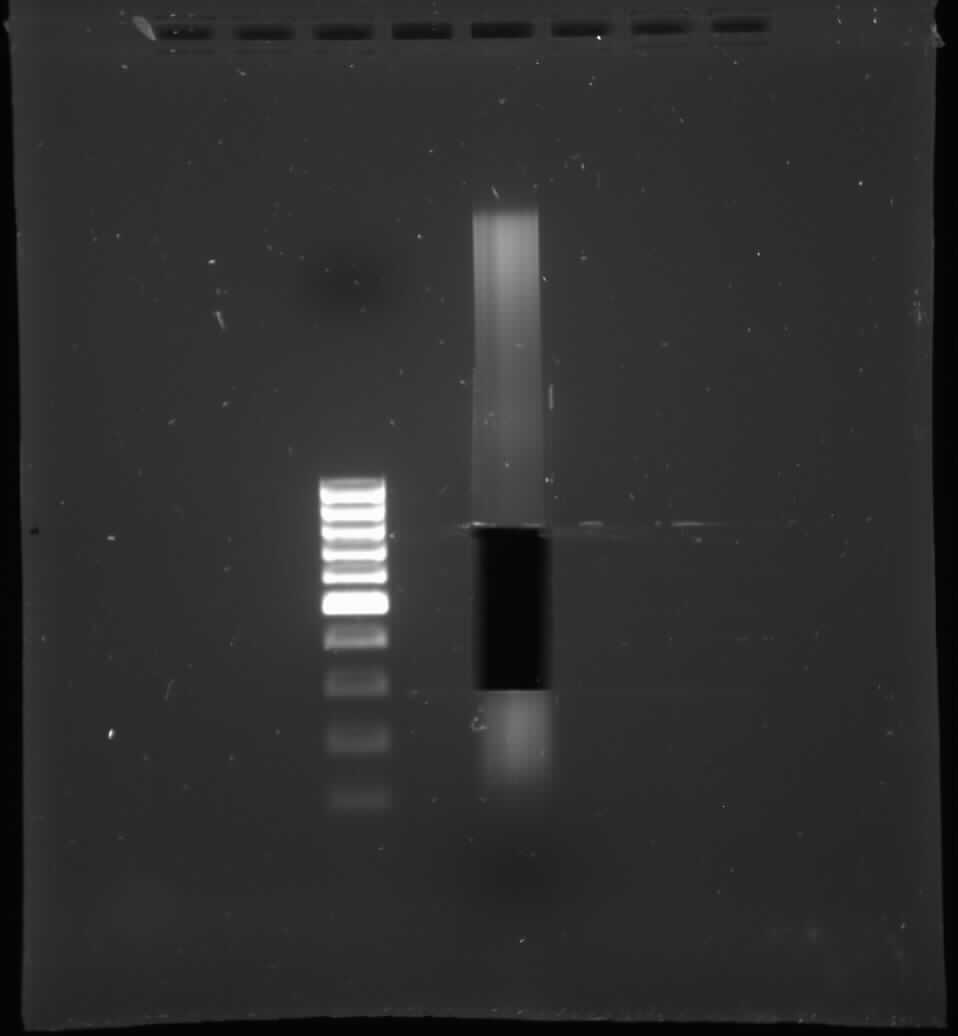
\includegraphics[scale=0.3]{GelSizeSelection_071011}
\caption{Gel picture after size selection.}
\label{SizeSel}
\end{center}
\end{figure}

%\begin{figure}[!htb]
%\begin{center}
%\subfigure[two pools sheared with the Covaris settings from Table \ref{Covaris}]{\label{shearedPools}\includegraphics[scale=0.32]{shearedPools_180610_1}}
%\hfill
%\subfigure[after size selection of the pools]{\label{shearedPools}\includegraphics[scale=0.3]{sizeSelection_after_250610}}
%\caption{Size selection of fragments after shearing.}
%\label{shearedPools}
%\end{center}
%\end{figure}

\subsection
{selective amplification}
\label{selAmp}
\begin{itemize}
\item save 6$\mu$l of the eluate of the last step for later qPCR
\item then set up a PCR with the remaining 24$\mu$l eluate:
	\begin{itemize}
	\item 6.0 $\mu$l H2O
	\item 50.0 $\mu$l 2x Phusion Mastermix \footnote{Do not use Phusion PCR kit with standard dNTP's. Phusion only works with high quality dNTP's !}
	\item 10.0 $\mu$l P1-thiol primer (10$\mu$M) $\rightarrow$ 1.0$\mu$M end concentration \footnote{I found that a much higher primer concentration than usual can greatly increase yield}
	\item 10.0 $\mu$l P2-thiol primer (10$\mu$M)
	\item 24 $\mu$l RAD library template
	\end{itemize}
\item split the PCR mix into 5x 20$\mu$l volumes and add 10$\mu$l mineral oil to each PCR tube
\item then run each tube with the PCR programme shown in table \ref{selPCR}
%%%%% ctable - for tables with footnotes. Very useful. 
% call ctable package
\ctable[ 
	caption = PCR programme,
	label = selPCR,
	pos = h,
	width = 45mm,
	center
]
{>{\centering}X>{\raggedright}X>{\raggedright}X}
{
	\tnote{30sec per kb recommended}
}
{
					\FL
98$^{\circ}$  & 30sec	 &	 \ML
98$^{\circ}$  & 10sec	 & 
\multirow{3}{*}{\Huge{$\}$}\normalsize$\times$18} \NN
65$^{\circ}$  & 30sec	 &	\NN
72$^{\circ}$  & 30sec\tmark[a] &\ML 
72$^{\circ}$ & 5min	&	\NN
4$^{\circ}$  & $\infty$	&	\LL
}
\end{itemize}

\subsection
{purifcation and concentration of the selective PCR product}
\begin{itemize}
\item {\color{red}use filter-tips or different pipettes for anything post-PCR !}
\item combine all PCR products and check 5$\mu$l of it on a 1.25\% gel next to 2$\mu$l Genruler
\item take 6$\mu$l of the PCR product for qPCR
\item purify the rest of the PCR product over a MinElute column eluting with 10$\mu$l EB
\end{itemize}

\subsection
{determination of template amount used for selective PCR by qPCR}
\begin{itemize}
\item {\color{red}use filter-tips}
\item use 4$\mu$l of the 6$\mu$l of the PCR product set aside in the previous step to determine it's DNA concentration with the fluorometer and picoGreen dye and use it as a standard in the qPCR
\item make 8x 1:10 serial dilutions of the PCR product in 10$\mu$l EB each to produce a standard curve
\item set up 20$\mu$l qPCR reactions with SybrGreen PCR master mix and 2$\mu$l template: 
	\begin{itemize}
	\item three replicates of serial dilutions including negative control
	\item three replicates of the template saved in step \ref{selAmp}
	\end{itemize}
\item from the C$_{t}$ values and the known amount of template molecules in the standard dilution, determine the amount of template molecules per locus and individual \footnote{This can be used to predict the expected proportion of false homozygote genotype calls due to PCR drift and false heterozygote genotype calls due to high coverage PCR mutations.} \\(see \texttt{sRAD/qPCR/TRIAL\_LIB\_241011\_data.xls})
\end{itemize}


\subsection
{normalisation of the library}
Unless the library looks like a homogeneous smear on the gel, it is advisable to normalise it.
\begin{itemize}
\item check activity of double strand specific nuclease (DSN) with control template from the kit
\item {\color{red}use filter-tips}
\item take 6$\mu$l of the purified PCR product and add 2$\mu$l 4x Hybridization buffer \footnote{500mM final NaCl concentration for annealing. EB contains 10mM Tris-HCl at pH 8.5, 1x hybridization buffer contains 50mM HEPES at pH 7.5. So the pH in the mixture should be close to 7.5.}
\item put 4$\mu$l of the mixture in each of two tubes, labeled ``1/8'' and ``1/16''
\item overlay the reaction mixtures with 10$\mu$l mineral oil and spin down for 2 min at max speed
\item in a thermal cycler, heat the mixture to 98$^{\circ}$ for 2 min
\item \ldots then incubate at 68$^{\circ}$ for 5 hours
\item put DSN master buffer into thermal cycler to preheat it to 68$^{\circ}$
\item make a 1/8th and 1/16 dilution of the DSN enzyme with DSN storage buffer
\item keep the thermal cycler at 68$^{\circ}$C and add 5$\mu$l preheated DSN master buffer to each tube while keeping the tube in the cycler, then flick, spin down briefly and immediately put back into the thermal cycler 
\item incubate for 10 minutes at 68$^{\circ}$C 
\item add 1$\mu$l of 1/8th or 1/16th DSN enzyme into each tube respectively \footnote{just add the enzyme, don't flick, don't spin down, just be quick, i. e. no more than 10 seconds for this step!}
\item incubate for 25 minutes at 68$^{\circ}$C 
\item add 10$\mu$l DSN stop solution, mix and spin \footnote{the reaction mixture contains 5mM MgCl$_{2}$ and the stop solution contains 5mM EDTA to neutralise it. Figure 4(B) in the TRIMMER kit manual suggests that inactivation of DSN by heating is not guaranteed to be complete.}
\end{itemize}

\subsection
{test PCR of normalisation}
\begin{itemize}
\item {\color{red}use filter-tips}
\item from each vial of the last step (i. e. ``1/8'' and ``1/16''), set up three 10$\mu$l test PCR's with 1$\mu$l template
\item run PCR for 5, 10 and 15 cycles with temperature steps as in table \ref{selPCR} and check 5$\mu$l PCR product on a 1.25\% EtBr gel next to 2$\mu$l Genruler
\item examine the PCR product: homogeneous smear in right size range?, 5 cycle PCR product visible? (see figure \ref{NormTestPCR})

\begin{figure}[!htb]
\begin{center}
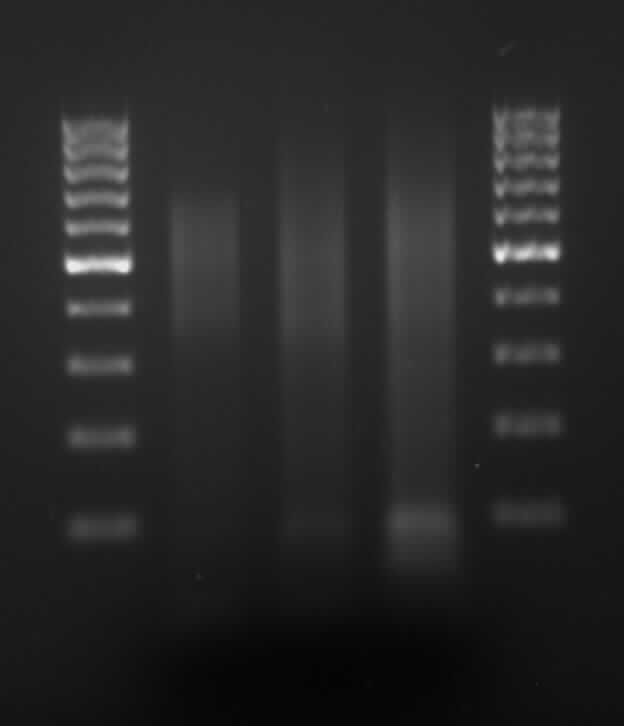
\includegraphics[scale=0.4]{Normalisation_test_lib_PCR_28072011}
\caption{Gel picture of 5, 10 and 15 cycle test PCR's (from left to right).}
\label{NormTestPCR}
\end{center}
\end{figure}

\item decide which DSN dissolution produced the better result
\end{itemize}

\subsection
{amplification of normalised library}
\begin{itemize}
\item {\color{red}use filter-tips}
\item set up a 50$\mu$l PCR as follow:
	\begin{itemize}
	\item 25$\mu$l 2x Phusion Master mix
	\item 5$\mu$l P1-thiol primer (10$\mu$M)
	\item 5$\mu$l P2-thiol primer (10$\mu$M)
	\item 10$\mu$l normalised library
	\item 5$\mu$l ddH$_{2}$O
	\end{itemize}
\item run the PCR programme in table \ref{selPCR} for 5-7 cycles, depending on the outcome of the test PCR \footnote{These additional PCR cycles do not further bias the library's representation of the pre-normalisation template since this PCR starts with a lot of template molecules as indicated by the few cycles necessary to create a visible PCR product.}
\end{itemize}

\subsection
{purification of the library}
\begin{itemize}
\item {\color{red}use filter-tips}
\item purify the 50$\mu$l PCR product over a MinElute column
\item elute with 25$\mu$l EB
\item use 4$\mu$l for DNA concentration measurement with fluorometer
\item calculate an estimate of the molar concentration of the library
\end{itemize}

%\begin{figure}[!htb]
%\begin{center}
%\includegraphics[scale=0.5]{selPCR_260610_cropped}
%\caption{PCR products of test amplifications of two libraries left of their respective templates. Adapter dimers are visible at $\sim$130bp.}
%\label{testAmp}
%\end{center}
%\end{figure}

%\subsubsection
%{perform a 100$\mu$l PCR}
%\begin{itemize}
%\item with 4$\mu$l template if very strong PCR product from test PCR, otherwise up to 30$\mu$l template
%\item 18 PCR cycles only in order to minimize PCR duplicates and bias
%\item purify the PCR product with Qiagen MinElute PCR purification column, elute with 20$\mu$l
%\item use filter-tips for anything post-PCR !
%\end{itemize}
%
%\subsubsection
%{gel purification of amplified library}
%\begin{itemize}
%\item use filter-tips for anything post-PCR !
%\item rinse the gel tank and use fresh buffer before running the gel if you have run a different library before
%\item run elution (20$\mu$l) in one lane of 1.25\% agarose gel with 10 $\mu$l 6X Orange Dye for 1h 15 min at 6.7 V/cm
%\item the wells should be less than half full, otherwise migration of fragments will be distorted \footnote{5--6mm wide wells}
%\item load 20$\mu$l 100bp ladder (20$\mu$g) in the left lane, leave 1 lane space between standard and library
%\item use fresh razor blade and UV transilluminator (long wave setting to minimize mutations) to cut out a size range of $\sim$350-750 bp \footnote{adapter dimers run at $\sim$130bp, when making the vertical cuts, be sure not to go below 350bp, otherwise risk of adapter dimer contamination (Maureen Liu)}
%\end{itemize}
%
%%\begin{figure}[!ht]%a picture has to be inserted into a figure environment in order to make it floatable; a star at figure has to be added for a two column layout
%%\begin{center}
%%\subfigure[before size selection]{\label{before}\includegraphics[scale=0.5]{selPCR_040710_gel_before_cropped}}
%%\hfill %pushes the graphics to the left and right margins
%%\subfigure[after size selection]{\label{after}\includegraphics[scale=0.5]{selPCR_040710_gel_after}}
%%\end{center}
%%\caption{Size selection of the amplified RAD library. Adapter dimer bands are clearly visible. About $\sim$0.03\% of the reads from this library came from adapter dimers or sequences with very small genomic inserts.}
%%\label{sizeSelection2}%the label command has to occur after the caption but inside the figure environment to refer (with \ref) to the figure and not the section of the document
%%\end{figure}
%
%
%\subsubsection
%{gel extraction}
%\begin{itemize}
%\item filter-tips !
%\item with MinElute Gel Extraction Kit
%\item melt agarose slice at room temperature with frequent mixing
%\item elute in 20 $\mu$l EB
%\end{itemize}
%
%
%
%\subsubsection
%{quantify molar concentration of RAD tags}
%\begin{itemize}
%\item determine DNA concentration of the library with fluorimeter twice and each with at least 3 replicates of the calf thymus standard serial dilution
%\item determine size distribution and peak size of RAD tags with Agilent Bioanalyzer 2100 DNA chip or from agarose gel picture
%\item multiply peak size by 650 [g/mol] \footnote{the molecular weight of a base pair} to get the molecular weight of the library
%\item divide the DNA concentration of the library [g/$\mu$l] by it's molecular weight to get the molar concentration [nmole/L] of RAD tags in the library
%\end{itemize}
%
\subsection
{validate library \protect \footnote{optional because of the cost and effort involved with cloning, but recommended before spending a lot of money on Solexa sequencing}}
\begin{itemize}
\item A-tail PCR product
\item T/A clone 1.0 $\mu$l of library into pGEM vector
\item Sanger sequence a few dozen clones
\item check for whether the sequences contain a P1 adapter sequence on one end and a P2 adapter sequence on the other
%\item also check for the frequency of PCR duplicates among the clones\footnote{when P2Y adapter is at the same position in two clone sequences} and blast the sequences
\end{itemize}

\pagebreak

\begin{landscape}

\ctable[ 
	caption =  {comparison among different ddRADseq protocols},
	label = compProt,
%	pos = htb!,
%	sideways,
	width = 240mm,
	captionskip = 1ex, % bring the caption closer to the table
	doinside=\footnotesize,
	center,
]
{l>{\raggedright}X>{\raggedright}X>{\raggedright}X>{\raggedright}X>{\raggedright}X>{\raggedright}X>{\raggedright}X}
{
}
{
\FL
\textbf{protocol}   &   \textbf{adapters}   &   \textbf{DNA isolation}   &   \textbf{digestion}   &   \textbf{ligation}   &   \textbf{gel size selection}   &   \textbf{PCR}   &   \textbf{purification}
\ML
\cite{Peterson2012}		& P1 and P2 adapter at stock conc. of 40$\mu$M, short adapters and long PCR primers	& NA	& digest for 3h, no heat-inact. -- instead bead puri.	& 30min ligation at RT, 2-10 fold excess of adapters to sticky ends	& before PCR, automated DNA size selection with Pippin-Prep (Sage Science)	& 20ng size-selected library per PCR reaction, 2$\mu$M end conc. of each PCR primer, only 8-12 cycles (?!) 	& AMPure beads \NN % the ``\rowcolor'' command requires the ``colortbl'' packageted
\rowcolor[gray]{0.9} \cite{Andolfatto2011}		& 10$\mu$M stock conc., short adapters + long PCR primers	& Puregene (Qiagen)	& 10ng DNA per sample, with 3.3U of 4bp cutter MseI (i. e. no double-digerst), 3h at 37$^{\circ}$C followed by heat-inact.	& 5nmole adapters, only 1 U of T4 DNA ligase in a volume of 50$\mu$l, 1h at 16$^{\circ}$C 	& before PCR, ladder mixed into library, 2\% gel	& only 15 cycles, Phusion	& AMPure beads \NN
\cite{Parchman2012}		& 1$\mu$M stock conc. for P1 (EcoRI) adapter, 
					10$\mu$M stock conc. for P2 (MseI) adapter, 
					annealing in pure water (?!), 
					short adapters + long PCR primers	& NA	& 6- and 4bp cutter, 10U EcoRI, only 1U MseI, digestion in T4 buffer, 
														NaCl added to $\sim$50mM end conc.,
														volume 9$\mu$l, 8h, heat-inact.		& 1pmole EcoRI adapter, 10pmole MseI adapter, 
																						67 NEB units T4 ligase, 6h at 16$^{\circ}$C, 
																						ligation in only 11.4$\mu$l 				& after PCR, 2.5\% gel, low electric field gel runs,
																															EtBr gels, many lanes					&  individual PCR before pooling samples and before gel size selection,
																													   											30 cycles (?!), only 0.08$\mu$M end conc. of each primer in PCR (?!),
																																								BioRad Iproof High Fidelity DNA polymerase						& QiaQuick spin columns \NN
\rowcolor[gray]{0.9} Kerth et al. (2030) & &	&	&	&	&	&\NN
\LL
}

\end{landscape}

%\bibliographystyle{apalike}
%\bibliography{/Users/Claudius/Documents/MyLiterature/Literature}




% 
%\begin{enumerate}
%\item Implement a new random genetic marker technique called \textit{sRAD}.
%\item Find loci linked to Dobzhansky-Muller incompatibilities responsible for  sterility in F$_{1}$ male hybrids of two grasshopper subspecies.
%\end{enumerate}
%
%\begin{itemize}
%\item How many genes are responsible for the observed hybrid male sterility? 
%\item Are these genes disproportionately located on the X-chromosome?
%\end{itemize}
%
%
%\subsubsection{Background}
%Two subspecies of \emph{Chorthippus parallelus} -- \emph{Chorthippus parallelus parallelus} and \emph{C. p. erythropus} -- form a hybrid zone in the Pyrenees. F$_{1}$ male hybrids between \emph{C. p. parallelus} and \emph{C. p. erythropus} from outside the hybrid zone are almost completely sterile with degenerate testes and a severely disrupted meiosis \citep{Hewitt1987}
%$\sim$1800 RAD tags 
% \textsterling1,100.
%(see section \ref{QTL cross} on p. \pageref{QTL cross}),
%\citep[p. 284-319]{CoyneOrr2004}, such as: 
%
%
%\begin{figure*}[htb]%a picture has to be inserted into a figure environment in order to make it floatable; a star at figure has to be added for a two column layout
%\begin{center}
%\subfigure[Oscillogramm (bottom) and traces of the corresponding hindleg movements (top) of a singing \emph{C. montanus} male. Three syllables are shown. (from \citealp{Helversen1994}, p. 271) ]{\label{montanus}\includegraphics[scale=1.0]{montanus}}
%\hfill %pushes the graphics to the left and right margins
%\subfigure[Syllable duration over body temperature in \emph{C. parallelus} (syn. \emph{longicornis}) and \emph{C. montanus} males. (from \citealp{Helversen1987}, p. 121)]{\label{syllable}\includegraphics[scale=1.2]{syllableDuration}}
%\end{center}
%\caption{The songs of \emph{C. montanus} and \emph{C. parallelus} differ only in the duration of their syllables.}
%\label{songdiff}%the label command has to occur after the caption but inside the figure environment to refer (with \ref) to the figure and not the section of the document
%\end{figure*}
%
%
%
%%%% sRAD sketch from Floragenex website
%\begin{figure*}[tbp]
%\begin{center}
%\includegraphics[scale=.25]{RADprocessOverview}
%\caption{\emph{sRAD} is basically Solexa/illumina sequencing of restriction fragment ends. Each restriction site defines the position of two tightly linked RAD tags.} 
%\label{Floragenex}
%\end{center}
%\end{figure*}
%%%%
%
%\underline{s}equenced \underline{R}estriction \underline{S}ite associated \underline{D}NA.
%
%50\% NERC funding 
%
%
%
%
%
%%%% my own sketch of the sRAD library preparation process
%\begin{figure*}[htbp]
%\begin{center}
%\includegraphics[scale=.6]{sRADprocessSketch}
%\caption{(a) The genome is cut but a restriction endonuclease ~~(b) P1 adapters (blue) containing a different 5base pair long nucleotide sequence (red) for each individual sample are ligated to restriction fragment ends. ~~(c) After pooling the P1 ligated samples, they are sheared to below 1kb before a size range is selected on the gel. The shearing step makes the marker technique repeatable. ~~(d) A few steps further, the P2 adapter, a divergent Y adapter, is ligated onto all fragments. In the following PCR, only fragments with at least one P1 adapter will be amplified. ~~(e) Further complexity reduction by restricting the library with frequent cutter restriction enzymes. ~~(f) Solexa sequencing. The first 5 base pairs in the reads identify the individual. A T/A single nucleotide polymorphism is marked by the red frames.} 
%\label{sRADsketch}
%\end{center}
%\end{figure*}
%%%%
%
%
%\begin{quotation}
%``\ldots the most important determinant of [QTL analysis] power is F2 and/or backcross sample size \ldots  small samples sizes lead to systematic overestimation of QTL addititive effects, the so-called \textsc{beavis} effect \ldots simulations suggest that this effect becomes small as experimental sample sizes near $\sim$500 genotyped and phenotyped individuals.'' \citep{Orr2001a} 
%\end{quotation}
%
%The temperature curve in the CT room where the grasshoppers have been recorded is oscillating by 2$^{\circ}$C 
%
%
%
%%%%%%%% PCA table
%% Requires the booktabs package if the memoir class is not being used
%\begin{table}[!htbp]
%\begin{center}
%\topcaption{correlation of peaks with PCA scores} % requires the 'topcapt' package
%\begin{tabular}{@{}lcr@{}}
%\toprule
%& \multicolumn{2}{c}{scaling by:}\\
%& Peak & Individual\\
%\cmidrule(l){2-3} % Partial rule. (r) trims the line a little bit on the right; (l) & (lr) also possible
%& Comp.1 & Comp.1\\
%\midrule
%Peak.1  & -0.8809&-0.8237\\
%Peak.2  & -0.8249&-0.8490\\
%Peak.3  & -0.7623&-0.8563\\
%Peak.4  & -0.8255&-0.6677\\
%Peak.5 & -0.8886&-0.5243\\
%Peak.6  &-0.4218&0.3017\\
%Peak.7  &-0.8427&0.1139\\
%Peak.8  &-0.6538&0.4732\\
%Peak.9  &-0.9358&0.3918\\
%Peak.10&-0.7138&-0.3078\\
%Peak.11 &-0.7750&0.1455\\
%Peak.12& -0.8784&-0.4255\\
%Peak.13 &-0.8469&0.1801\\
%Peak.14 &-0.8413&0.5327\\
%Peak.15 &-0.8619&0.5204\\
%Peak.16 &-0.8038&0.4222\\
%Peak.17 &-0.8171&0.2868\\
%Peak.18 &-0.8320&0.4565\\
%Peak.19 &-0.8707&0.6411\\
%Peak.20 &-0.8834&0.6679\\
%Peak.21 &-0.8377&0.6844\\
%Peak.22& -0.8207&0.6334\\
%Peak.23 &-0.7635&0.5860\\
%\bottomrule
%\end{tabular}
%\label{PCcorrPeak}
%\end{center}
%\end{table}
%%%%%%% PCA table
%
%
%
%\begin{table*} % the asterisk puts the table on that page, I don't know why, but here it fits better
%\centering
%\topcaption{MANOVA results for species difference of CHC blends among females using data scaled by peak.} % the top caption needs to be before the begin{tabular} command
%\begin{tabular}{@{}lrrrrrr@{}}
%\toprule
%& \small{Df} & \small{Pillai} & \small{approx F} & \small{num Df} & \small{den Df} & {Pr($>$F)}\\  
%\midrule  
%\small{Species} & \small{1} & \small{0.817}  &   \small{6.19}    & \small{23}    & \small{32} & \small{1.9e-06***}\\
%\small{Residuals}  &   \small{54} & & & & & \\                                       
%\bottomrule
%\end{tabular}
%\label{manova}
%\end{table*}
%
%
%
%%%%% multivariate outlier individuals
%\begin{table}[!htbp]
%\centering
%\topcaption{Multivariate outlier individuals.} % requires the 'topcapt' package
%\begin{tabular}{@{}lr@{}}
%\toprule
%Individual & $\sqrt[2]{Mahanalobis}$\\
%\midrule
%26parF & 7.066\\
%49parF & 7.025\\
%50parF & 5.999\\
%52parF & 7.186\\
%53parF & 5.976\\
%55parF & 6.740\\
%85parF & 6.819\\
%29monF\underline{}Fin & 6.349\\
%32monF\underline{}Fin & 6.059\\
%84monF\underline{}Fin & 6.871\\
%61monF\underline{}Ger & 5.938\\
%\bottomrule
%\end{tabular}
%\label{outlier}
%\end{table}
%
%
%
%\bibliographystyle{apalike}
%\onecolumn
%\setlength{\columnsep}{20pt}
%\begin{multicols}{2} 
%% the separation of the columns has been set in the preambel
%%\begin{multicols}{2}
%
%\bibliography{/Users/Claudius/Documents/MyLiterature/Literature}
%
%\end{multicols}
%

%\end{document}

\include{Appendix2/appendix2}

\end{appendices}

% *************************************** Index ********************************
\printthesisindex % If index is present

\end{document}
